% ============================================================================
% Solving CT Heterogeneous Agent Models: PINNs and Deep Learning
% University of Geneva
% April 20--23 & May 4--7, 2026
% Duration: 75 minutes
% ============================================================================

\documentclass[aspectratio=169,11pt]{beamer}

% ---------- Theme and colors ----------
\usecolortheme{dove}
\setbeamertemplate{navigation symbols}{}
\setbeamertemplate{footline}{%
  \hfill\usebeamerfont{page number in head/foot}%
  \usebeamercolor[fg]{normal text}%
  \insertframenumber\,/\,\inserttotalframenumber\kern1em\vskip4pt}
\setbeamerfont{frametitle}{size=\huge}

% ---------- Packages ----------
\usepackage[utf8]{inputenc}
\usepackage[T1]{fontenc}
\usepackage{amsmath,amssymb,amsfonts}
\usepackage{bm}
\usepackage{graphicx}
\usepackage{tikz}
\usetikzlibrary{shapes,arrows.meta,positioning,calc,fit,backgrounds,patterns,decorations.pathreplacing}
\usepackage{pgfplots}
\pgfplotsset{compat=1.18}
\usepackage{booktabs}
\usepackage{hyperref}
\usepackage{multicol}
\usepackage{xcolor}
\usepackage{algorithm}
\usepackage{algorithmic}
\usepackage{listings}
\usepackage{pifont}

% ---------- Listings style for Python ----------
\lstset{
    language=Python,
    basicstyle=\footnotesize\ttfamily,
    keywordstyle=\color{uzhblue}\bfseries,
    commentstyle=\color{uzhgreydark}\itshape,
    stringstyle=\color{darkgreen},
    showstringspaces=false,
    breaklines=true,
    frame=none,
    xleftmargin=0pt,
    aboveskip=2pt,
    belowskip=2pt,
    escapeinside={(*@}{@*)},
}

% ---------- Custom colors ----------
\definecolor{uzhblue}{rgb}{0,0,0.5}
\definecolor{uzhgreylight}{RGB}{236,238,241}
\definecolor{uzhgreydark}{RGB}{81,86,94}
\definecolor{harvardcrimson}{RGB}{153,0,0}
\definecolor{unil@blue}{RGB}{0,140,204}
\definecolor{unil@black}{RGB}{35,31,32}
\definecolor{darkgreen}{RGB}{0,100,0}
\definecolor{darkred}{RGB}{139,0,0}
\definecolor{softblue}{RGB}{70,130,180}
\definecolor{softorange}{RGB}{230,159,0}
\definecolor{softgreen}{RGB}{0,158,115}

% ---------- Set beamer colors ----------
\setbeamercolor{frametitle}{bg=uzhgreylight, fg=uzhblue}
\setbeamercolor{title}{fg=uzhblue}
\setbeamercolor{structure}{fg=uzhblue}
\setbeamercolor{block title}{bg=unil@blue, fg=white}
\setbeamercolor{block body}{bg=uzhgreylight}
\setbeamercolor{block title alerted}{bg=darkred,fg=white}
\setbeamercolor{block body alerted}{bg=red!5}
\setbeamercolor{block title example}{bg=darkgreen,fg=white}
\setbeamercolor{block body example}{bg=green!5}
\setbeamercolor{item}{fg=unil@black}
\setbeamercolor{normal text}{fg=unil@black}

% ---------- Emphasis and hyperlinks ----------
\newcommand{\emphc}[1]{\textcolor{harvardcrimson}{#1}}
\hypersetup{colorlinks,linkcolor=harvardcrimson,urlcolor=harvardcrimson}

% ---------- Reduce vertical spacing ----------
\setlength{\parskip}{0pt}

% ---------- Math commands ----------
\newcommand{\R}{\mathbb{R}}
\newcommand{\E}[1]{\mathbb{E}\!\left[#1\right]}
\DeclareMathOperator*{\argmin}{arg\,min}
\DeclareMathOperator*{\argmax}{arg\,max}
\newcommand{\ud}{\,\mathrm{d}}
\newcommand{\ubar}[1]{\underline{#1}}

% ---------- Title ----------
\title[Deep Learning -- Geneva 2026]%
{Deep Learning for Economics and Finance}
\subtitle{Solving CT Heterogeneous Agent Models:\\From Finite Differences to PINNs and EMINNs}
\author{Simon Scheidegger}
\institute[HEC Lausanne]{HEC, University of Lausanne}
\date{University of Geneva\\April 20--23 \& May 4--7, 2026}

\begin{document}

% ============================================================================
% PART 0: TITLE & OUTLINE
% ============================================================================

% --- Slide 1: Title ---
{\setbeamercolor{background canvas}{bg=uzhgreylight}
\begin{frame}
\titlepage
\vspace{-0.4cm}
\begin{center}
{\footnotesize Based on: Achdou, Han, Lasry, Lions \& Moll (2022), \emph{Rev.\ Econ.\ Stud.}\ 89(1), 45--86.}\\[2pt]
{\footnotesize Gu, Lauriere, Merkel \& Payne (2024), ``Global Solutions to Master Equations.'' arXiv:2406.13726.}\\[2pt]
{\footnotesize Self-contained slides; Python implementations are introduced after the theory.}\\[4pt]
{\footnotesize Materials: \url{https://github.com/sischei/Deep_Learning_for_Solving_And_Estimating_Dynamic_Economic_Models}}
\end{center}
\end{frame}
}

% --- Slide 2: Recap and Goals ---
\begin{frame}{Recap and Goals}
\textbf{From Deck 1} (this morning): We derived the \emphc{theory} of CT heterogeneous agent models:
\begin{itemize}\itemsep2pt
    \item Stochastic calculus: Brownian motion, It\^o's lemma, Poisson jumps
    \item KFE (Fokker--Planck): density evolution, from physics to economics
    \item HJB: optimal consumption-savings policy
    \item Equilibrium: coupled HJB + KFE + market clearing (Huggett, Aiyagari, KS)
    \item Master equation: single PDE encoding the full equilibrium
\end{itemize}

\vspace{0.4em}
\textbf{This deck}: How to \emphc{solve} these models numerically.
\begin{enumerate}\itemsep3pt
    \item \textbf{Part I}: Traditional approach (finite differences) --- brief overview, limitations
    \item \textbf{Part II}: \emphc{PINNs for the coupled HJB + KFE system} (stationary: Huggett/Aiyagari)
    \item \textbf{Part III}: \emphc{EMINNs for the master equation} (with aggregate shocks: Krusell--Smith)
    \item \textbf{Part IV}: Results, comparison, and the ``deep learning conundrum''
\end{enumerate}
\end{frame}

% --- Slide 3: Table of Contents ---
\begin{frame}{Table of Contents}
\tableofcontents[hideallsubsections]
\end{frame}

% ============================================================================
% PART I: FINITE DIFFERENCES (BRIEF)
% ============================================================================

\section{Traditional Approach: Finite Differences}

\begin{frame}{}
\vfill
\begin{center}
{\Huge \textcolor{uzhblue}{\textbf{Part I}}}\\[12pt]
{\LARGE Traditional Approach: Finite Differences}\\[6pt]
{\large The Benchmark We Want to Beat}
\end{center}
\vfill
\end{frame}

% --- Slide: FD Overview ---
\begin{frame}{Finite Differences: The Classical Approach}
\small
\textbf{How have economists traditionally solved these models?}

\vspace{0.2em}
\begin{columns}[T]
\column{0.55\textwidth}
\textbf{Finite difference method} (Achdou et al., 2022):
\begin{enumerate}\itemsep1pt
    \item Discretize wealth $a$ on a grid $\{a_1, \ldots, a_I\}$
    \item Approximate derivatives by finite differences:
    \[
    V'(a_i) \approx \frac{V_{i+1} - V_i}{\Delta a} \quad \text{or} \quad \frac{V_i - V_{i-1}}{\Delta a}
    \]
    \item \emphc{Upwind scheme}: use forward diff.\ when savings $> 0$, backward when $< 0$
    \item Iterate HJB $\to$ policy $\to$ KFE $\to$ aggregates $\to$ prices $\to$ HJB
\end{enumerate}

\column{0.42\textwidth}
\begin{center}
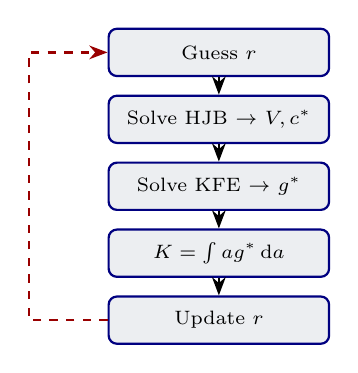
\begin{tikzpicture}[
    box/.style={rectangle, rounded corners=3pt, draw=uzhblue, thick, fill=uzhgreylight, minimum width=2.8cm, minimum height=0.6cm, align=center, font=\scriptsize},
    arrow/.style={-Stealth, thick}
]
\node[box] (guess) at (0,3) {Guess $r$};
\node[box] (hjb) at (0,2.15) {Solve HJB $\to$ $V, c^*$};
\node[box] (kfe) at (0,1.3) {Solve KFE $\to$ $g^*$};
\node[box] (mc) at (0,0.45) {$K = \int ag^*\ud a$};
\node[box] (update) at (0,-0.4) {Update $r$};

\draw[arrow] (guess) -- (hjb);
\draw[arrow] (hjb) -- (kfe);
\draw[arrow] (kfe) -- (mc);
\draw[arrow] (mc) -- (update);
\draw[arrow, dashed, harvardcrimson] (update.west) -- +(-1.0,0) |- (guess.west);
\end{tikzpicture}
\end{center}
\end{columns}

\vspace{0.1em}
{\footnotesize This summarizes the finite-difference workflow; code examples are provided later in Python.}
\end{frame}

% --- Slide: FD Results ---
\begin{frame}{Finite Differences: What They Produce}
\footnotesize
\begin{columns}[T]
\column{0.48\textwidth}
\textbf{Finite-Difference Example: Aiyagari GE}\\[1pt]
The classical FD approach solves:
\begin{itemize}\itemsep0pt
    \item HJB block: upwind discretization + implicit updates
    \item KFE block: transition operator + stationary distribution
    \item Price block: root-finding for market-clearing $r$
\end{itemize}

\vspace{0.15em}
\textbf{Produces:}
\begin{itemize}\itemsep0pt
    \item Value function $V(a, n)$
    \item Consumption/savings policy $c^*(a, n)$
    \item Stationary density $g^*(a, n)$
    \item Equilibrium prices $r^*, w^*$
\end{itemize}

\vspace{0.15em}
\emphc{This is our ground truth} for validating deep learning methods.

\column{0.48\textwidth}
\begin{center}
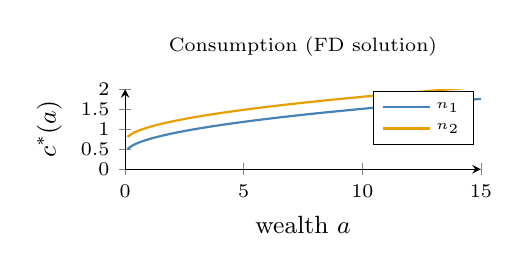
\begin{tikzpicture}
\begin{axis}[
    width=6.1cm, height=2.6cm,
    xlabel={\small wealth $a$}, ylabel={\small $c^*(a)$},
    xmin=0, xmax=15, ymin=0, ymax=2,
    axis lines=left,
    tick label style={font=\scriptsize},
    label style={font=\normalsize},
    title={\scriptsize Consumption (FD solution)},
    title style={at={(0.5,1.08)}},
    legend style={at={(0.98,0.3)}, anchor=south east, font=\tiny},
]
\addplot[softblue, thick, domain=0.1:15, samples=60]
    {0.4 + 0.35*sqrt(x)};
\addlegendentry{$n_1$}
\addplot[softorange, thick, domain=0.1:15, samples=60]
    {0.7 + 0.35*sqrt(x)};
\addlegendentry{$n_2$}
\end{axis}
\end{tikzpicture}

\vspace{0.15em}
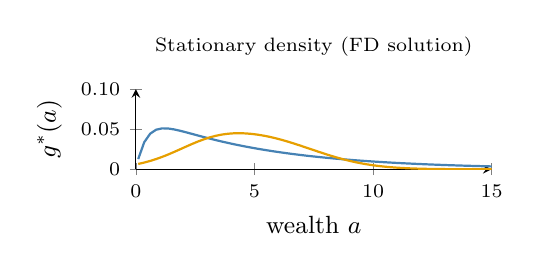
\begin{tikzpicture}
\begin{axis}[
    width=6.1cm, height=2.6cm,
    xlabel={\small wealth $a$}, ylabel={\small $g^*(a)$},
    xmin=0, xmax=15, ymin=0, ymax=0.1,
    axis lines=left,
    scaled y ticks=false,
    ytick={0,0.05,0.10},
    yticklabels={0,0.05,0.10},
    tick label style={font=\scriptsize},
    label style={font=\normalsize},
    title={\scriptsize Stationary density (FD solution)},
    title style={at={(0.5,1.08)}},
]
\addplot[softblue, thick, domain=0.1:15, samples=60]
    {0.07*exp(-0.2*(x-0.1)) * (1 - exp(-2*x))};
\addplot[softorange, thick, domain=0.1:15, samples=60]
    {0.04*exp(-(x-5)^2/12) + 0.01*exp(-(x-3)^2/4)};
\end{axis}
\end{tikzpicture}
\end{center}
\end{columns}
\end{frame}

% --- Slide: FD Limitations ---
\begin{frame}{Why Finite Differences Are Not Enough}
\footnotesize
\begin{columns}[T]
\column{0.48\textwidth}
\textbf{FD works well for:}
\begin{itemize}\itemsep1pt
    \item[\textcolor{darkgreen}{\ding{51}}] Stationary HJB--KFE systems
    \item[\textcolor{darkgreen}{\ding{51}}] Low-dimensional states $(a,n)$
    \item[\textcolor{darkgreen}{\ding{51}}] Monotone convergence theory
    \item[\textcolor{darkgreen}{\ding{51}}] Fast sparse linear algebra
\end{itemize}

\column{0.48\textwidth}
\textbf{FD is strained by:}
\begin{itemize}\itemsep1pt
    \item[\textcolor{darkred}{\ding{55}}] Global KS master equation
    \item[\textcolor{darkred}{\ding{55}}] State $(a,n,z,g)$ with distribution $g$
    \item[\textcolor{darkred}{\ding{55}}] Dense tensor-product grids
    \item[\textcolor{darkred}{\ding{55}}] Moment truncation of $g$
\end{itemize}
\end{columns}

\vspace{0.4em}
\begin{alertblock}{Takeaway}
Neural methods do not remove the equilibrium conditions; they approximate
value and distribution maps without building a full grid over $g$.
\end{alertblock}
\end{frame}

% ============================================================================
% PART II: PINNs FOR HJB + KFE
% ============================================================================

\section{PINNs for HJB + KFE}

\begin{frame}{}
\vfill
\begin{center}
{\Huge \textcolor{uzhblue}{\textbf{Part II}}}\\[12pt]
{\LARGE PINNs for the Coupled HJB + KFE System}\\[6pt]
{\large Solving Huggett and Aiyagari with Neural Networks}
\end{center}
\vfill
\end{frame}

% --- Slide: PINN Recap ---
\begin{frame}{Recap: What Is a PINN?}
\textbf{From Block 1 (earlier today)}: A \emphc{Physics-Informed Neural Network} (PINN) solves a PDE by:
\begin{enumerate}\itemsep2pt
    \item Parameterizing the solution by a neural network: $u(x) \approx \mathcal{N}_\theta(x)$
    \item Computing PDE \emphc{residuals} via \emphc{automatic differentiation}
    \item Minimizing the residual over \emphc{collocation points} (no grid needed!)
\end{enumerate}

\vspace{0.2em}
\begin{center}
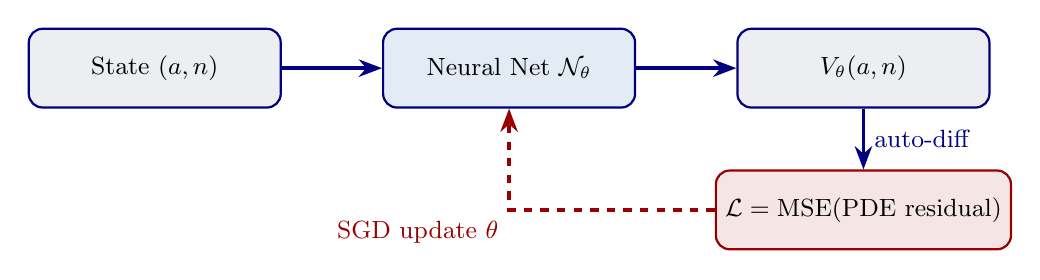
\begin{tikzpicture}[
    box/.style={rectangle, rounded corners=5pt, draw=uzhblue, thick, fill=uzhgreylight,
                 minimum width=3.2cm, minimum height=1cm, align=center, font=\small},
    arrow/.style={-Stealth, very thick, uzhblue}
]
\node[box] (input) at (0,0) {State $(a, n)$};
\node[box, fill=softblue!15] (nn) at (4.5,0) {Neural Net $\mathcal{N}_\theta$};
\node[box] (output) at (9,0) {$V_\theta(a,n)$};
\node[box, fill=harvardcrimson!10, draw=harvardcrimson] (loss) at (9,-1.8) {$\mathcal{L} = \text{MSE}(\text{PDE residual})$};

\draw[arrow] (input) -- (nn);
\draw[arrow] (nn) -- (output);
\draw[arrow] (output) -- node[right, font=\small] {auto-diff} (loss);
\draw[arrow, dashed, harvardcrimson] (loss.west) -| node[below left, font=\small] {SGD update $\theta$} (nn.south);
\end{tikzpicture}
\end{center}

\vspace{0.1em}
\textbf{Key advantage}: \emphc{mesh-free} --- no grid needed, scales to high dimensions.
\end{frame}

% ====================================================================
% PE Stepping Stones (before the full GE Aiyagari model)
% ====================================================================

% --- Slide: Partial Equilibrium Stepping Stones ---
\begin{frame}{Partial Equilibrium HJB: Stepping Stones}
\small
Before tackling full GE (Aiyagari), solve the HJB alone with exogenous prices.

\begin{columns}[T]
\column{0.48\textwidth}
\begin{block}{Discrete Income (1D)}
\begin{itemize}\itemsep1pt
  \item 2-state Markov chain $z\in\{z_L,z_H\}$
  \item Coupled system: $V_1(a), V_2(a)$
  \item FOC eliminates $\max$; upwind FD vs PINN
  \item \textbf{Notebook 01}
\end{itemize}
\end{block}

\column{0.48\textwidth}
\begin{block}{OU Diffusion (2D)}
\begin{itemize}\itemsep1pt
  \item Earnings: $dz = \theta(\mu-z)\,dt + \sigma\,dW$
  \item Single PDE: $V(a,z)$, second-order in $z$
  \item Neumann BCs; 2D auto-diff PINN
  \item \textbf{Notebook 02}
\end{itemize}
\end{block}
\end{columns}

\vspace{0.3em}
\centering
\textbf{Key insight}: PINNs scale gracefully from 1D$\to$2D --- no grid explosion.
\end{frame}

% ====================================================================
% PE Model 1: Discrete Income (3 slides)
% ====================================================================

% --- Slide: PE Discrete — Model and HJB ---
\begin{frame}{PE Discrete Income: Model and HJB}
\small
\begin{columns}[T]
\column{0.50\textwidth}
\textbf{Setup} (exogenous prices $r,w$):
\begin{itemize}\itemsep1pt
  \item CRRA utility $u(c)=\frac{c^{1-\gamma}}{1-\gamma}$, discount $\rho$
  \item Budget: $\dot{a}=r\,a+w\,z-c$, \; $a\ge\ubar{a}$
  \item Income: 2-state Markov chain $z\in\{z_L,z_H\}$\\
        with Poisson rates $\lambda_{12},\lambda_{21}$
\end{itemize}

\vspace{0.3em}
\textbf{FOC} eliminates $\max$:
\[
  u'(c)=V_j'(a) \;\Longrightarrow\;
  \boxed{c_j^*=(V_j')^{-1/\gamma}}
\]

\column{0.48\textwidth}
\textbf{Coupled HJB} for states $j=1,2$:
\[
\boxed{
  \rho\,V_j = u(c_j^*)
            + V_j'\,s_j
            + \lambda_{jk}(V_k-V_j)
}
\]
where $s_j = r\,a + w\,z_j - c_j^*$ is \emphc{savings}.

\vspace{0.3em}
\textbf{Boundary conditions:}
\begin{itemize}\itemsep1pt
  \item $a=\ubar{a}$: enforce $s_j=r\ubar a+wz_j-c_j\ge0$.
  \item If binding: $c_j=r\ubar a+wz_j$ and boundary mass may form.
  \item $a=\bar{a}$: no outflow on truncated grid.
\end{itemize}
\end{columns}
\end{frame}

% --- Slide: PE Discrete — Upwind FD ---
\begin{frame}{PE Discrete Income: Upwind Finite-Difference Scheme}
\small
\begin{columns}[T]
\column{0.52\textwidth}
\begin{block}{Algorithm (implicit iteration)}
\begin{algorithmic}[1]
  \STATE Forward/backward FD of $V$:\\
         $V_a^F=(V_{i+1}-V_i)/\Delta a$,\;
         $V_a^B=(V_i-V_{i-1})/\Delta a$
  \STATE FOC inversion $\to$ consumption:\\
         $c^F=(V_a^F)^{-1/\gamma}$,\;$c^B=(V_a^B)^{-1/\gamma}$
  \STATE Savings candidates:\\
         $s^F=\text{inc}-c^F$,\; $s^B=\text{inc}-c^B$
  \STATE \emphc{Upwind selection}:\\
         $\mathbb{I}^F\!=\!(s^F\!>\!0)$,\;
         $\mathbb{I}^B\!=\!(s^B\!<\!0)\wedge\neg\mathbb{I}^F$
  \STATE Build generator\\
         $A = A_a(\text{upwind}) + \Lambda\otimes I_J$
  \STATE Implicit step:\\
         $\bigl(\tfrac{1}{\Delta}+\rho\bigr)V^{n+1}\!-\!A\,V^{n+1}=u(c)+\tfrac{V^n}{\Delta}$
\end{algorithmic}
\end{block}

\column{0.46\textwidth}
\textbf{Key design choices:}
\begin{itemize}\itemsep2pt
  \item \emphc{Upwind}: uses the derivative consistent with the drift direction $\to$ numerical stability
  \item \emphc{Kronecker stacking}: $\Lambda\otimes I_J$ couples the two income states into one $2J\times 2J$ system
  \item \emphc{Implicit}: unconditionally stable; large $\Delta$ accelerates convergence
  \item Converges in ${\sim}13$ iterations to $\|V^{n+1}-V^n\|_\infty < 10^{-8}$
\end{itemize}

\vspace{0.2em}
{\scriptsize\textit{Reference: Achdou et al.\ (2022, REStud), Appendix~B.}}
\end{columns}
\end{frame}

% --- Slide: PE Discrete — PINN ---
\begin{frame}[fragile]{PE Discrete Income: PINN Approach}
\small
\begin{columns}[T]
\column{0.52\textwidth}
\textbf{Network architecture:}\\[2pt]
1 input ($a$) $\to$ 4$\times$64 \texttt{tanh} $\to$ 2 outputs ($V_1,V_2$)

\vspace{0.3em}
\textbf{Loss components:}\\[2pt]
\begin{tabular}{@{}lp{4.2cm}@{}}
\toprule
Term & Description \\
\midrule
$\mathcal{L}_{\text{PDE}}$ & HJB residual MSE (both states) \\
$\mathcal{L}_{\text{BC}}$  & Dirichlet at $\ubar{a},\bar{a}$ (from FD) \\
$\mathcal{L}_{\text{curv}}$ & Concavity: $\text{relu}(V'')^2$ \\
\bottomrule
\end{tabular}

\vspace{0.3em}
\textbf{Key code} (auto-diff):
\begin{lstlisting}
V = net(a)          # [N, 2]
V_a = grad(V.sum(), a)  # V'
c = V_a ** (-1/gamma)   # FOC
s = income - c
R = rho*V - u(c) - V_a*s
    - lam*(V_swap - V)   # residual
\end{lstlisting}

\column{0.42\textwidth}
\begin{center}
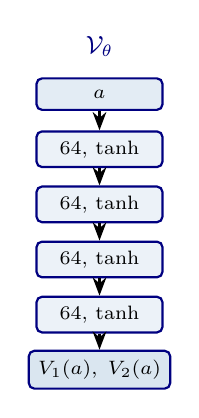
\begin{tikzpicture}[
    layer/.style={rectangle, rounded corners=2pt, draw=uzhblue, thick,
                  minimum width=1.6cm, minimum height=0.4cm, align=center,
                  font=\scriptsize},
    arrow/.style={-Stealth, thick}
]
\node[font=\small\bfseries, uzhblue] at (0,4.0) {$\mathcal{V}_\theta$};
\node[layer, fill=softblue!15] (in)  at (0,3.4) {$a$};
\node[layer, fill=softblue!10] (h1)  at (0,2.7) {64, $\tanh$};
\node[layer, fill=softblue!10] (h2)  at (0,2.0) {64, $\tanh$};
\node[layer, fill=softblue!10] (h3)  at (0,1.3) {64, $\tanh$};
\node[layer, fill=softblue!10] (h4)  at (0,0.6) {64, $\tanh$};
\node[layer, fill=softblue!20] (out) at (0,-0.1) {$V_1(a),\;V_2(a)$};

\draw[arrow] (in)  -- (h1);
\draw[arrow] (h1)  -- (h2);
\draw[arrow] (h2)  -- (h3);
\draw[arrow] (h3)  -- (h4);
\draw[arrow] (h4)  -- (out);
\end{tikzpicture}
\end{center}

\vspace{0.2em}
{\scriptsize No grid, no upwind logic --- auto-diff handles all derivatives.}
\end{columns}
\end{frame}

% ====================================================================
% PE Model 2: OU Diffusion (3 slides)
% ====================================================================

% --- Slide: PE Diffusion — Model and 2D HJB ---
\begin{frame}{PE Diffusion Income: Model and 2D HJB}
\small
\begin{columns}[T]
\column{0.50\textwidth}
\textbf{Earnings process} (Ornstein--Uhlenbeck):
\[
\boxed{dz = \theta(\mu - z)\,dt + \sigma\,dW}
\]
with mean-reversion $\theta$, long-run mean $\mu$, volatility $\sigma$.

\vspace{0.3em}
\textbf{2D HJB} (after FOC substitution):
\[
\boxed{
  \rho\,V = u(c^*) + V_a\,s
          + \theta(\mu\!-\!z)\,V_z
          + \tfrac{1}{2}\sigma^2 V_{zz}
}
\]
where $c^*=(V_a)^{-1/\gamma}$, $s=r\,a+w\,z-c^*$.

\vspace{0.2em}
\emphc{Key difference from 1D}: the second-order diffusion term $V_{zz}$.

\column{0.46\textwidth}
\textbf{Domain \& boundary conditions:}

\vspace{0.2em}
{\centering\scriptsize
\begin{tabular}{@{}r@{\;}l@{}}
\textcolor{darkred}{\textbf{Left/right}} ($a$): & Neumann $V_a = u'(\text{inc})$ \\
\textcolor{softblue}{\textbf{Top/bottom}} ($z$): & Reflecting $V_z = 0$ \\
\end{tabular}
\par}

\vspace{0.3em}
\begin{center}
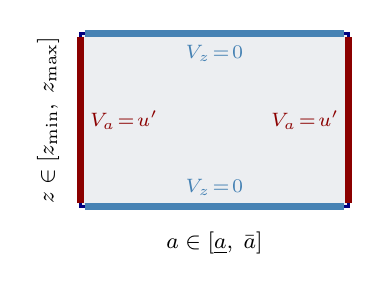
\begin{tikzpicture}[font=\scriptsize]
  % Domain rectangle
  \draw[very thick, uzhblue, fill=uzhgreylight]
    (0,0) rectangle (3.4,2.2);
  % Axis labels along edges
  \node[below, font=\footnotesize] at (1.7, -0.2)
    {$a \in [\ubar{a},\;\bar{a}]$};
  \node[left, rotate=90, anchor=south, font=\footnotesize] at (-0.15, 1.1)
    {$z \in [z_{\min},\;z_{\max}]$};
  % Left/right BC: colored edge highlights + labels inside
  \draw[darkred, line width=2.5pt] (0,0.05) -- (0,2.15);
  \draw[darkred, line width=2.5pt] (3.4,0.05) -- (3.4,2.15);
  \node[darkred, font=\scriptsize] at (0.55, 1.1) {$V_a\!=\!u'$};
  \node[darkred, font=\scriptsize] at (2.85, 1.1) {$V_a\!=\!u'$};
  % Top/bottom BC: colored edge highlights + labels inside
  \draw[softblue, line width=2.5pt] (0.05,2.2) -- (3.35,2.2);
  \draw[softblue, line width=2.5pt] (0.05,0) -- (3.35,0);
  \node[softblue, font=\scriptsize] at (1.7, 1.95) {$V_z\!=\!0$};
  \node[softblue, font=\scriptsize] at (1.7, 0.25) {$V_z\!=\!0$};
\end{tikzpicture}
\end{center}
\end{columns}
\end{frame}

% --- Slide: PE Diffusion — 2D FD Scheme ---
\begin{frame}[shrink=3]{PE Diffusion: 2D Finite-Difference Scheme}
\small
\begin{columns}[T]
\column{0.50\textwidth}
\textbf{Operator splitting by dimension:}

\vspace{0.1em}
\emphc{Wealth direction} ($a$): upwind as in 1D
\begin{itemize}\itemsep0pt
  \item Forward/backward FD, FOC, upwind selection
  \item Produces sparse $A_a$ (block-diagonal in $z$)
\end{itemize}

\vspace{0.1em}
\emphc{Earnings direction} ($z$):
\begin{itemize}\itemsep0pt
  \item Drift $\theta(\mu-z)$: \emphc{upwind} FD
  \item Diffusion $\frac{1}{2}\sigma^2 V_{zz}$: \emphc{central} FD
  \item Reflecting BCs: ghost-point symmetry\\
        {\scriptsize ($V_{-1}=V_1$ at $z_{\min}$, $V_{J_z}=V_{J_z-2}$ at $z_{\max}$)}
  \item Produces $A_z$ of size $J_z\times J_z$
\end{itemize}

\vspace{0.1em}
\textbf{Combined generator:}
\[
  A = A_a(s) + A_z \otimes I_{J_a}
\]

\column{0.46\textwidth}
\textbf{Implicit step} (same structure as 1D):
\[
  \Bigl(\tfrac{1}{\Delta}+\rho\Bigr)V^{n+1} - A\,V^{n+1}
  = u(c) + \tfrac{V^n}{\Delta}
\]

\vspace{0.1em}
\textbf{Grid scaling:}
\begin{center}
\begin{tabular}{@{}lcc@{}}
\toprule
& Classroom & Production \\
\midrule
$J_a$ & 50 & 200 \\
$J_z$ & 30 & 100 \\
Unknowns & 1,500 & 20,000 \\
\bottomrule
\end{tabular}
\end{center}

\vspace{0.1em}
\textbf{Performance:}
\begin{itemize}\itemsep0pt
  \item Converges in ${\sim}9$ implicit iterations
  \item Sparse direct solve (scipy \texttt{spsolve})
  \item Cost grows as $O(J_a \times J_z)$ --- manageable in 2D, but \emphc{explodes in 3D+}
\end{itemize}
\end{columns}
\end{frame}

% --- Slide: PE Diffusion — 2D PINN ---
\begin{frame}[fragile]{PE Diffusion: 2D PINN}
\small
\begin{columns}[T]
\column{0.52\textwidth}
\textbf{Network}: 2 inputs $(a,z)$ $\to$ 4$\times$64 \texttt{tanh} $\to$ 1 output $V$

\vspace{0.3em}
\textbf{Key ingredient} --- nested auto-diff for $V_{zz}$:
\begin{lstlisting}
V    = net(a, z)
V_a  = grad(V, a)    # wealth
V_z  = grad(V, z)    # earnings
V_zz = grad(V_z, z)  # diffusion!
\end{lstlisting}

\vspace{0.3em}
\textbf{Loss components} (same structure as 1D):
\begin{tabular}{@{}lp{4.0cm}@{}}
\toprule
Term & Description \\
\midrule
$\mathcal{L}_{\text{PDE}}$ & 2D HJB residual MSE \\
$\mathcal{L}_{\text{BC}}$  & Dirichlet on all 4 edges \\
$\mathcal{L}_{\text{curv}}$ & Concavity: $\text{relu}(V_{aa})^2$ \\
\bottomrule
\end{tabular}

\column{0.42\textwidth}
\begin{center}
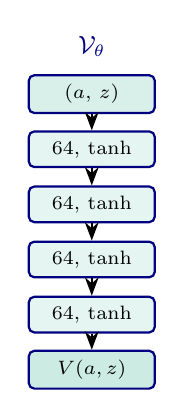
\begin{tikzpicture}[
    layer/.style={rectangle, rounded corners=2pt, draw=uzhblue, thick,
                  minimum width=1.6cm, minimum height=0.4cm, align=center,
                  font=\scriptsize},
    arrow/.style={-Stealth, thick}
]
\node[font=\small\bfseries, uzhblue] at (0,4.0) {$\mathcal{V}_\theta$};
\node[layer, fill=softgreen!15] (in)  at (0,3.4) {$(a,\,z)$};
\node[layer, fill=softgreen!10] (h1)  at (0,2.7) {64, $\tanh$};
\node[layer, fill=softgreen!10] (h2)  at (0,2.0) {64, $\tanh$};
\node[layer, fill=softgreen!10] (h3)  at (0,1.3) {64, $\tanh$};
\node[layer, fill=softgreen!10] (h4)  at (0,0.6) {64, $\tanh$};
\node[layer, fill=softgreen!20] (out) at (0,-0.1) {$V(a,z)$};

\draw[arrow] (in)  -- (h1);
\draw[arrow] (h1)  -- (h2);
\draw[arrow] (h2)  -- (h3);
\draw[arrow] (h3)  -- (h4);
\draw[arrow] (h4)  -- (out);
\end{tikzpicture}
\end{center}

\vspace{0.2em}
\colorbox{uzhgreylight}{\parbox{0.95\linewidth}{\centering\scriptsize
\textbf{1D $\to$ 2D}: add $z$ as 1 extra input neuron.\\
No grid explosion --- collocation cost is \emphc{dimension-free}.}}
\end{columns}
\end{frame}

% ====================================================================
% Transition slide: PE → GE
% ====================================================================

% --- Slide: From Partial to General Equilibrium ---
\begin{frame}{From Partial to General Equilibrium}
\small
\begin{center}
\begin{tabular}{@{}l c c c@{}}
\toprule
& \textbf{PE Discrete (NB\,01)} & \textbf{PE Diffusion (NB\,02)} & \textbf{GE Aiyagari (NB\,03)} \\
\midrule
PDEs solved     & HJB only   & HJB only   & HJB + KFE \\
Prices $(r,w)$  & exogenous  & exogenous  & \emphc{endogenous} \\
Income process  & 2-state Markov & OU diffusion & 2-state Markov \\
State dimension & 1D ($a$)   & 2D ($a,z$) & 1D ($a$) + GE loop \\
PINN networks   & $V_\theta$ only & $V_\theta$ only & $V_\theta$ + $g_\phi$ \\
FD unknowns     & $2J$       & $J_a \times J_z$ & $2J$ + distribution \\
\bottomrule
\end{tabular}
\end{center}

\vspace{0.2em}
\textbf{Progression of complexity:}
\begin{enumerate}\itemsep0pt
  \item \textbf{NB\,01}: isolate the HJB with simplest income process $\to$
        learn upwind FD and PINN mechanics
  \item \textbf{NB\,02}: extend to 2D with diffusion $\to$
        mesh-free PINN advantage ($V_{zz}$ via auto-diff)
  \item \textbf{NB\,03}: add the \emphc{KFE} for stationary distribution +
        \emphc{market clearing} $\to$ full Aiyagari GE
\end{enumerate}

\vspace{0.1em}
\centering
\colorbox{uzhgreylight}{\parbox{0.75\textwidth}{\centering\small
Notebook~03 adds the KFE and equilibrium conditions $\to$ \emphc{full Aiyagari}.}}
\end{frame}

% --- Slide: From Single PDE to Coupled System ---
\begin{frame}{From Single PDE to Coupled System}
\small
\textbf{Block 1 (PINNs)}: Solve a \emph{single} PDE (Poisson, HJB cake-eating, Black--Scholes).

\vspace{0.2em}
\textbf{Block 2 (this block)}: Solve a \emph{coupled system} of PDEs arising from equilibrium:

\vspace{0.2em}
\begin{center}
\small
\renewcommand{\arraystretch}{1.3}
\begin{tabular}{lll}
\toprule
\textbf{Component} & \textbf{PDE} & \textbf{Unknown} \\
\midrule
HJB (backward) & $\rho V = \max_c\{u(c) + V'\cdot s + \lambda(\Delta V)\}$ & Value $V(a,n)$ \\
KFE (forward) & $0 = -\partial_a[s\cdot g] - \lambda g + \lambda\hat{g}$ & Density $g(a,n)$ \\
Market clearing & $K = \sum_n \int a\,g\ud a$ & Prices $r, w$ \\
\bottomrule
\end{tabular}
\end{center}

\vspace{0.2em}
\textbf{The coupling}: HJB output ($c^* \to s$) is the KFE input (drift).\\
KFE output ($g \to K, L$) determines prices ($r, w$) that enter HJB.

\vspace{0.2em}
\begin{center}
\colorbox{uzhgreylight}{\parbox{0.7\textwidth}{\centering\small
\textbf{PINN approach}: Parameterize \emph{both} $V$ and $g$ by neural networks.\\
Minimize \emph{all} residuals \emphc{jointly} via a single loss function.}}
\end{center}
\end{frame}

% --- Slide: Formal Stationary System ---
\begin{frame}{Formal Target System (Stationary, Truncated Domain)}
\footnotesize
Train on $a\in[\ubar{a},\bar{a}]$, $n\in\{n_1,n_2\}$.
\[
\rho V=\max_c\left\{u(c)+V_a(wn+ra-c)+\lambda(n)\big(V(a,\hat n)-V(a,n)\big)\right\},\quad
c^*=(V_a)^{-1/\gamma}
\]
\[
0=-\partial_a\!\big[s(a,n)g(a,n)\big]-\lambda(n)g(a,n)+\lambda(\hat n)g(a,\hat n),\quad
s=wn+ra-c^*
\]

\vspace{-0.2em}
\begin{columns}[T]
\column{0.49\textwidth}
\textbf{Boundary/state constraints:}
\[
V_a(\ubar a,n)\ge u'(wn+r\ubar a),\qquad s(\ubar a,n)\ge 0
\]
\[
J(a,n):=s(a,n)g(a,n),\qquad J(\ubar a,n)=0
\]

\column{0.49\textwidth}
\textbf{Market clearing:}
\[
\text{Huggett: }\sum_n\int_{\ubar b}^{\bar b} b\,g(b,n)\ud b = 0
\]
\[
\text{Aiyagari: }K^s=\sum_n\int_{\ubar a}^{\bar a} a\,g(a,n)\ud a=K^d(r)
\]
\[
\sum_n\int_{\ubar a}^{\bar a}g(a,n)\ud a=1
\]
\end{columns}
\end{frame}

% --- Slide: PINN Architecture for Aiyagari ---
\begin{frame}{PINN Architecture for Aiyagari/Huggett}
\small
\begin{columns}[T]
\column{0.55\textwidth}
\textbf{Two neural networks:}
\begin{itemize}\itemsep1pt
    \item $V_\theta(a, n)$: value function network
    \begin{itemize}\itemsep0pt
        \item Input: $(a, n)$ \quad ($n$ encoded as 0/1)
        \item Output: scalar $V$
        \item Architecture: 3--4 hidden layers, 64 neurons, $\tanh$
    \end{itemize}
    \item $g_\phi(a, n)$: density network
    \begin{itemize}\itemsep0pt
        \item Input: $(a, n)$
        \item Output: scalar $g \geq 0$ (use softplus)
        \item Same architecture
    \end{itemize}
\end{itemize}

\vspace{0.2em}
\textbf{Derived quantities} (via auto-diff):
\begin{itemize}\itemsep1pt
    \item $V'_\theta = \partial_a V_\theta$ \quad $\Rightarrow$ consumption: $c^* = (V'_\theta)^{-1/\gamma}$
    \item $\partial_a g_\phi$ \quad $\Rightarrow$ KFE residual
\end{itemize}

\column{0.42\textwidth}
\begin{center}
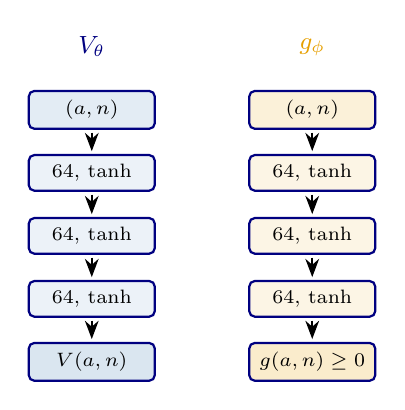
\begin{tikzpicture}[
    layer/.style={rectangle, rounded corners=2pt, draw=uzhblue, thick, minimum width=1.6cm, minimum height=0.4cm, align=center, font=\scriptsize},
    arrow/.style={-Stealth, thick, shorten >=1pt, shorten <=1pt}
]
% Value network
\node[font=\small\bfseries, uzhblue] at (0,4.4) {$V_\theta$};
\node[layer, fill=softblue!15] (v_in) at (0,3.6) {$(a, n)$};
\node[layer, fill=softblue!10] (v_h1) at (0,2.8) {64, $\tanh$};
\node[layer, fill=softblue!10] (v_h2) at (0,2.0) {64, $\tanh$};
\node[layer, fill=softblue!10] (v_h3) at (0,1.2) {64, $\tanh$};
\node[layer, fill=softblue!20] (v_out) at (0,0.4) {$V(a,n)$};

\draw[arrow] (v_in) -- (v_h1);
\draw[arrow] (v_h1) -- (v_h2);
\draw[arrow] (v_h2) -- (v_h3);
\draw[arrow] (v_h3) -- (v_out);

% Density network
\node[font=\small\bfseries, softorange] at (2.8,4.4) {$g_\phi$};
\node[layer, fill=softorange!15] (g_in) at (2.8,3.6) {$(a, n)$};
\node[layer, fill=softorange!10] (g_h1) at (2.8,2.8) {64, $\tanh$};
\node[layer, fill=softorange!10] (g_h2) at (2.8,2.0) {64, $\tanh$};
\node[layer, fill=softorange!10] (g_h3) at (2.8,1.2) {64, $\tanh$};
\node[layer, fill=softorange!20] (g_out) at (2.8,0.4) {$g(a,n) \geq 0$};

\draw[arrow] (g_in) -- (g_h1);
\draw[arrow] (g_h1) -- (g_h2);
\draw[arrow] (g_h2) -- (g_h3);
\draw[arrow] (g_h3) -- (g_out);
\end{tikzpicture}
\end{center}
\end{columns}
\end{frame}

% --- Slide: Explicit-policy formulation ---
\begin{frame}{Explicit-Policy HJB PINN: $\mathcal{N}_\theta(a,n) \to (V, c)$}
\small
The cleaner formulation used in notebooks 06--07 makes the policy a network output, not a quantity hidden inside derivatives of $V$.
\vspace{-0.3em}
\[
\mathcal{N}_\theta(a, n) \;=\; \bigl(\,V_\theta(a, n),\; c_\theta(a, n)\,\bigr),
\qquad c_\theta = \mathrm{softplus}(\cdot) + \varepsilon \;>\; 0.
\]
The loss enforces \emphc{both} the HJB residual \emphc{and} the FOC consistency:
\vspace{-0.3em}
\[
\mathcal{L}^{\text{HJB}} =
\underbrace{\tfrac{1}{M}\sum_m R_{\text{HJB}}\bigl(a_m, n_m;\, V_\theta, c_\theta\bigr)^2}_{\text{interior PDE residual}}
\;+\;
\kappa_{\text{FOC}}\,\underbrace{\tfrac{1}{M}\sum_m \bigl(c_\theta(a_m,n_m)^{-\gamma} - V'_{\theta,a}(a_m,n_m)\bigr)^2}_{\text{first-order condition}}.
\]

\textbf{Why this is more teachable than $c = (V_a)^{-1/\gamma}$:}
\begin{itemize}\itemsep0pt
    \item The FOC is an \emphc{explicit residual} students can monitor.
    \item No early-training pathologies from $V_a \le 0$.
    \item Policy is a smooth network output, plots stable from epoch~1.
    \item FOC residual must vanish \emph{independently} of the HJB residual.
\end{itemize}

{\footnotesize Generalises to two states (nb.\ 06: $V_1, V_2, c_1, c_2$) and OU income (nb.\ 07: $V(a,z), c(a,z)$). Notebook 08 keeps $c=(V_a)^{-1/\gamma}$ and outputs $(V,g)$ for the coupled HJB--KFE system.}
\end{frame}

% --- Slide: Loss Function ---
\begin{frame}[shrink=5]{PINN Objective: Interior + Boundary + Equilibrium}
\small
The total loss combines \emphc{all equilibrium conditions}:
\[
\boxed{
\mathcal{L}=
\kappa_{\text{HJB}}\mathcal{L}_{\text{HJB}}^{\text{int}}
+\kappa_{\text{KFE}}\mathcal{L}_{\text{KFE}}^{\text{int}}
+\kappa_{\text{KFE,cum}}\mathcal{L}_{\text{KFE}}^{\text{cum}}
+\kappa_{\text{SC}}\mathcal{L}_{\text{SC}}
+\kappa_{\text{flux}}\mathcal{L}_{\text{flux}}
+\kappa_{\text{mass}}\mathcal{L}_{\text{mass}}
+\kappa_{\text{MC}}\mathcal{L}_{\text{MC}}
}
\]

\vspace{0.1em}
\begin{center}
\scriptsize
\renewcommand{\arraystretch}{1.25}
\begin{tabular}{lll}
\toprule
\textbf{Component} & \textbf{Definition} & \textbf{What it enforces} \\
\midrule
$\mathcal{L}_{\text{HJB}}^{\text{int}}$ & $\frac{1}{M}\sum_m |R_{\text{HJB}}(a_m,n_m)|^2$ & Interior HJB \\[2pt]
$\mathcal{L}_{\text{KFE}}^{\text{int}}$ & $\frac{1}{M}\sum_m |R_{\text{KFE}}(a_m,n_m)|^2$ & Interior KFE \\[2pt]
$\mathcal{L}_{\text{KFE}}^{\text{cum}}$ & $\frac{1}{I}\sum_k |R_{\text{KFE}}^{\text{cum}}(a_k)|^2$ & Integrated KFE balance \\[2pt]
$\mathcal{L}_{\text{SC}}$ & $\sum_n\max(0,-s_\theta(\ubar a,n))^2$ & State constraint \\[2pt]
$\mathcal{L}_{\text{flux}}$ & $\sum_n(J(\ubar a,n)^2+J(\bar a,n)^2)$ & Boundary fluxes \\[2pt]
$\mathcal{L}_{\text{mass}}$ & $\left(\sum_n\int g_\phi\ud a-1\right)^2$ & Normalization \\[2pt]
$\mathcal{L}_{\text{MC}}$ & Huggett: $(\int b g)^2$; Aiyagari: $(K^s-K^d(r))^2$ & Market clearing \\
\bottomrule
\end{tabular}
\end{center}

\vspace{0.1em}
Softplus output enforces $g_\phi\ge 0$. Weights can be adapted with ReLoBRaLo.
\end{frame}

% --- Slide: HJB Residual ---
\begin{frame}[fragile]{HJB Residual: Computed via Auto-Differentiation}
\small
The interior HJB residual at collocation point $(a, n)$.  In notebook 08, consumption is recovered from the value derivative, $c^* = (V'_\theta)^{-1/\gamma}$.  In notebooks 06--07, replace $c^*$ by $c_\theta$ and add the explicit FOC residual from the previous slide.
\vspace{-0.3em}
\[
R_{\text{HJB}}(a,n) = \rho V_\theta - u(c^*) - V'_\theta \cdot (wn + ra - c^*) - \lambda(n)\big(V_\theta(a,\hat{n}) - V_\theta(a,n)\big)
\]
\vspace{-0.5em}
\begin{lstlisting}
def hjb_residual(model_V, a, n, r, w, params):
    a.requires_grad_(True)
    V = model_V(a, n)
    V_a = torch.autograd.grad(V, a, (*@\ldots@*))[0]  # auto-diff
    c_star = V_a.clamp(min=1e-8) ** (-1.0 / gamma)  # FOC
    s = w * n + r * a - c_star  # savings
    V_hat = model_V(a, n_hat)  # value in other state
    res = rho * V - u(c_star) - V_a * s
          - lam(n) * (V_hat - V)
    return res
\end{lstlisting}
\end{frame}

% --- Slide: Integrated / cumulative KFE residual ---
\begin{frame}{Integrated KFE: A Stable Companion}
\footnotesize
Differentiating a noisy density $g_\phi$ pointwise is fragile; cumulative probability balance is often more stable.

\vspace{0.2em}
\textbf{Local (strong-form) residual.}
\vspace{-0.3em}
\[
R_{\text{KFE}}(a,n) = \partial_a\!\bigl[s\,g_\phi\bigr] + \lambda(n)g_\phi(a,n) - \lambda(\hat n)g_\phi(a,\hat n).
\]
Wiggles in $g_\phi$ produce large $\partial_a$ noise.

\vspace{0.2em}
\textbf{Integrated flux balance} on a deterministic grid $\{a_k\}$, with $J_j=s_jg_j$:
\vspace{-0.3em}
\[
\begin{aligned}
R_{1,k}^{\text{cum}}
&= J_1(a_k)-J_1(\ubar a)
   + \int_{\ubar a}^{a_k}\!\bigl[\lambda_{12}g_1(u)-\lambda_{21}g_2(u)\bigr]\,\ud u,\\
R_{2,k}^{\text{cum}}
&= J_2(a_k)-J_2(\ubar a)
   + \int_{\ubar a}^{a_k}\!\bigl[\lambda_{21}g_2(u)-\lambda_{12}g_1(u)\bigr]\,\ud u.
\end{aligned}
\]
No $\partial_a g_\phi$; only quadrature.

\vspace{0.1em}
\begin{itemize}\itemsep0pt
    \item Cheap: one quadrature per epoch on a fixed grid.
    \item Improves stationary-density diagnostics in notebook 08.
    \item Use both: $\mathcal L^{\text{KFE}}=\kappa_{\text{loc}}\mathcal L_{\text{loc}}+\kappa_{\text{cum}}\mathcal L_{\text{cum}}$.
\end{itemize}
\end{frame}

% --- Slide: KFE Residual ---
\begin{frame}[fragile]{KFE Residual: Density Must Satisfy the Forward Equation}
\small
The interior stationary KFE residual at $(a, n)$:
\vspace{-0.3em}
\[
R_{\text{KFE}}(a,n) = \partial_a\!\big[s(a,n)\,g_\phi(a,n)\big] + \lambda(n)\,g_\phi(a,n) - \lambda(\hat{n})\,g_\phi(a,\hat{n})
\]
\vspace{-0.5em}
\begin{lstlisting}
def kfe_residual(model_g, model_V, a, n, r, w, params):
    a.requires_grad_(True)
    g = model_g(a, n)
    c_star = get_consumption(model_V, a, n, params)
    s = w * n + r * a - c_star
    flux = s * g  # flux = savings * density
    d_flux = torch.autograd.grad(flux, a, (*@\ldots@*))[0]
    g_hat = model_g(a, n_hat)  # density in other state
    res = d_flux + lam(n) * g - lam(n_hat) * g_hat
    return res
\end{lstlisting}
\end{frame}

% --- Slide: Boundary, Flux, and Clearing ---
\begin{frame}{Boundary, Flux, and Market-Clearing Terms}
\footnotesize
\textbf{Aiyagari market clearing}:
\vspace{-0.3em}
\[
\mathcal{L}_{\text{MC}} =
\left(\textstyle\sum_{n}\int_{\ubar a}^{\bar a}a\,g_\phi\ud a-K^{d}(r)\right)^2
\]
\vspace{-0.6em}
For Huggett replace with:
\[
\mathcal{L}_{\text{MC}}^{\text{H}}=\left(\textstyle\sum_n\int_{\ubar b}^{\bar b} b\,g_\phi(b,n)\ud b\right)^2.
\]

\vspace{-0.1em}
\textbf{Normalization}: \;
$\mathcal{L}_{\text{mass}} = \bigl(\sum_{n} \int_{\ubar{a}}^{\bar{a}} g_\phi(a,n)\ud a - 1\bigr)^2$

\vspace{0.05em}
\textbf{State-constraint penalty}:
\[
\mathcal{L}_{\text{SC}} = \sum_{n} \max\!\left(0,\; -s_\theta(\ubar{a}, n)\right)^2
\]

\vspace{-0.1em}
\textbf{Boundary flux penalty} (truncated domain $[\ubar a,\bar a]$):
\[
\mathcal{L}_{\text{flux}} = \sum_n\left(J_\phi(\ubar a,n)^2 + J_\phi(\bar a,n)^2\right),\qquad
J_\phi(a,n)=s_\theta(a,n)\,g_\phi(a,n)
\]
Integrals are evaluated via Monte Carlo or quadrature.
\end{frame}

% --- Slide: Training the PINN ---
\begin{frame}{Training Algorithm: Jointly Solving HJB + KFE}
\begin{columns}[T]
\column{0.52\textwidth}
\begin{block}{PINN Training (Stationary Equilibrium)}
\footnotesize
\setlength{\itemsep}{0pt}
\begin{algorithmic}[1]
\STATE Initialize $V_\theta$, $g_\phi$, guess $r^{(0)}$ \;\;\textit{(FD reserved for validation)}
\FOR{$k = 1, \ldots, N_{\text{epochs}}$}
    \STATE Sample $M$ collocation points $\{(a_m, n_m)\}$
    \STATE Compute $c_m^* = (V'_\theta(a_m))^{-1/\gamma}$
    \STATE Compute $R_{\text{HJB}}^m$, $R_{\text{KFE}}^m$ via auto-diff
    \STATE Integrate KFE on a fixed asset grid
    \STATE Compute $\mathcal{L}_{\text{SC}}, \mathcal{L}_{\text{flux}}, \mathcal{L}_{\text{mass}}, \mathcal{L}_{\text{MC}}$
    \STATE Total loss: $\mathcal{L} = \sum \kappa_i \mathcal{L}_i$;\; update $\theta,\phi$ (Adam)
    \IF{$k \mod N_r = 0$}
        \STATE $r \leftarrow r + \eta(K^s - K^d)$
    \ENDIF
\ENDFOR
\STATE Freeze collocation grid; run FP64 L-BFGS polish
\end{algorithmic}
\end{block}

\column{0.45\textwidth}
\footnotesize
\textbf{Key choices:}
\begin{itemize}\itemsep0pt
    \item \textbf{Collocation}: sample $(a,n)$ uniformly on $[\ubar{a}, \bar{a}] \times \{n_1, n_2\}$
    \item \textbf{Price update}: update $r$ slowly (every $N_r$ steps) to let NN adapt
    \item \textbf{Loss weights}: start with $\kappa_{\text{HJB}}=\kappa_{\text{KFE}}=1$, larger $\kappa_{\text{SC}},\kappa_{\text{flux}},\kappa_{\text{MC}}$
    \item \textbf{Optimizer}: Adam, lr $\sim 10^{-3}$, then FP64 L-BFGS
    \item \textbf{Validation}: compare against FD only after training
\end{itemize}

\vspace{0.15em}
\begin{center}
\colorbox{uzhgreylight}{\parbox{0.95\columnwidth}{\centering\scriptsize
Same philosophy as Day~5: \emphc{economic equations = loss function};
\emphc{auto-diff = all derivatives}.}}
\end{center}
\end{columns}
\end{frame}

% --- Slide: Huggett PINN ---
\begin{frame}{Applying the PINN: Huggett (1993) Model}
\small
\textbf{Huggett model} (endowment economy, zero net supply of bonds):

\vspace{0.2em}
\begin{columns}[T]
\column{0.50\textwidth}
\textbf{Differences from Aiyagari:}
\begin{itemize}\itemsep1pt
    \item Asset: risk-free bond $b$ (not capital)
    \item Budget: $db = (qb + n - c)\ud t$
    \item Market clearing: $\sum_n \int b\,g(b,n)\ud b = \emphc{0}$
    \item Price: bond return $q$ (not interest rate via firm FOC)
\end{itemize}

\vspace{0.2em}
\textbf{PINN modification:}
\begin{itemize}\itemsep1pt
    \item Same architecture ($V_\theta$, $g_\phi$)
    \item HJB: replace $ra$ by $qb$, remove wage
    \item $\mathcal{L}_{\text{MC}} = \left(\int b\,g_\phi\ud b\right)^2$
    \item Iterate on $q$ instead of $r$
\end{itemize}

\column{0.47\textwidth}
\begin{center}
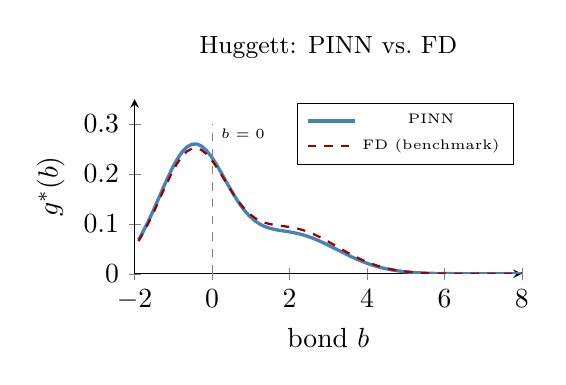
\begin{tikzpicture}
\begin{axis}[
    width=6.5cm, height=3.8cm,
    xlabel={bond $b$}, ylabel={$g^*(b)$},
    xmin=-2, xmax=8, ymin=0, ymax=0.35,
    axis lines=left,
    legend style={at={(0.98,0.98)}, anchor=north east, font=\tiny},
    title={\small Huggett: PINN vs.\ FD},
    title style={at={(0.5,1.08)}, font=\small},
]
% PINN solution
\addplot[softblue, very thick, domain=-1.9:8, samples=80]
    {0.25*exp(-(x+0.5)^2/1.5) + 0.08*exp(-(x-2)^2/3)};
\addlegendentry{PINN}
% FD solution (dashed)
\addplot[harvardcrimson, thick, dashed, domain=-1.9:8, samples=80]
    {0.24*exp(-(x+0.5)^2/1.5) + 0.09*exp(-(x-2)^2/3)};
\addlegendentry{FD (benchmark)}
\draw[gray, dashed] (axis cs:0,0) -- (axis cs:0,0.3);
\node[font=\tiny] at (axis cs:0.8,0.28) {$b=0$};
\end{axis}
\end{tikzpicture}
\end{center}

{\small PINN closely matches the FD benchmark.}
\end{columns}
\end{frame}

% --- Slide: Aiyagari PINN ---
\begin{frame}[shrink=15]{Applying the PINN: Aiyagari (1994) Model}
\small
\textbf{Aiyagari model} (production economy, capital market clearing):

\vspace{0.2em}
\begin{columns}[T]
\column{0.50\textwidth}
\textbf{vs.\ Huggett:} two prices $(r,w)$ from firm FOC, $\int a g = K$, $\int n g = L$, $r = \alpha K^{\alpha-1}L^{1-\alpha} - \delta$.

\vspace{0.3em}
\textbf{PINN diagnostics (notebook 08):}\\[2pt]
{\scriptsize
\renewcommand{\arraystretch}{1.0}
\begin{tabular}{@{}ll@{}}
\toprule
Diagnostic & Value \\
\midrule
$K^{\text{FD}}$ / $K^{\text{PINN}}$ & $0.30893$ / $0.30894$ \\
$|K^{\text{FD}}-K^{\text{PINN}}|$ & $8.7\!\times\!10^{-6}$ \\
$c$ MSE & $4.7\!\times\!10^{-4}$ \\
$g$ MSE & $8.1\!\times\!10^{-4}$ \\
KS dist.\ $z_1$/$z_2$ & $0.066$/$0.059$ \\
$\max|R_{\text{HJB}}|$ & $5.7\!\times\!10^{-2}$ \\
$\max|R_{\text{KFE}}|$ & $2.7\!\times\!10^{-1}$ \\
\bottomrule
\end{tabular}}

\vspace{0.2em}
{\footnotesize \emphc{Honest read:} $K$ matches to 5 digits; pointwise density and KS gaps are non-trivial. The integrated-KFE term targets exactly the loosest residual.}

\column{0.47\textwidth}
\begin{center}
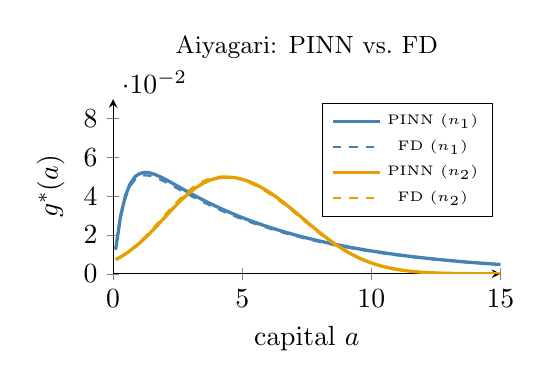
\begin{tikzpicture}
\begin{axis}[
    width=6.5cm, height=3.8cm,
    xlabel={capital $a$}, ylabel={$g^*(a)$},
    xmin=0, xmax=15, ymin=0, ymax=0.09,
    axis lines=left,
    legend style={at={(0.98,0.98)}, anchor=north east, font=\tiny},
    title={\small Aiyagari: PINN vs.\ FD},
    title style={at={(0.5,1.08)}, font=\small},
]
% PINN n1
\addplot[softblue, very thick, domain=0.1:15, samples=80]
    {0.07*exp(-0.18*(x-0.1)) * (1 - exp(-2*x))};
\addlegendentry{PINN ($n_1$)}
% FD n1
\addplot[softblue, thick, dashed, domain=0.1:15, samples=80]
    {0.068*exp(-0.18*(x-0.1)) * (1 - exp(-2*x))};
\addlegendentry{FD ($n_1$)}
% PINN n2
\addplot[softorange, very thick, domain=0.1:15, samples=80]
    {0.045*exp(-(x-5)^2/12) + 0.01*exp(-(x-3)^2/4)};
\addlegendentry{PINN ($n_2$)}
% FD n2
\addplot[softorange, thick, dashed, domain=0.1:15, samples=80]
    {0.044*exp(-(x-5)^2/12) + 0.012*exp(-(x-3)^2/4)};
\addlegendentry{FD ($n_2$)}
\end{axis}
\end{tikzpicture}
\end{center}

{\small Right-skewed, mass at $\ubar{a}$: reproduced by PINN.}
\end{columns}
\end{frame}

% --- Slide: Handling Borrowing Constraints ---
\begin{frame}{Handling the Borrowing Constraint}
\small
The borrowing constraint $a \geq \ubar{a}$ is a key challenge for PINNs.

\vspace{0.1em}
\begin{columns}[T]
\column{0.48\textwidth}
\begin{block}{Option A: Soft constraint (penalty)}
\footnotesize
Add penalty: $\psi(a) = -\tfrac{1}{2}\kappa(a - \ubar{a})^2$ for $a \leq \ubar{a}$

\vspace{0.1em}
Advantages:
\begin{itemize}\itemsep0pt
    \item Simple to implement
    \item Smooth loss landscape
    \item Avoids mass point issues in KFE
\end{itemize}
\end{block}

\column{0.48\textwidth}
\begin{block}{Option B: Hard constraint (trial solution)}
\footnotesize
Architecture: $V_\theta(a,n) = (a - \ubar{a})\hat{V}_\theta + V_{\text{BC}}$

\vspace{0.1em}
Advantages:
\begin{itemize}\itemsep0pt
    \item Exact BC satisfaction
    \item No tuning of $\kappa$
    \item Recall Day~5, Notebook~02
\end{itemize}
\end{block}
\end{columns}

\vspace{0.1em}
\textbf{Recommendation} (Achdou et al., 2022; Gu et al., 2024):
\begin{center}
\colorbox{uzhgreylight}{\parbox{0.8\textwidth}{\centering\footnotesize
Use the \emphc{soft borrowing constraint} $\psi(a)$. The inequality BC causes technical problems (non-differentiable $V$, mass point in $g$). Softening avoids these while being economically faithful for $\kappa$ large enough.}}
\end{center}
\end{frame}

% --- Slide: PINN for Huggett vs Aiyagari: Distributions ---
\begin{frame}[shrink=2]{PINN Solutions: Comparing Huggett and Aiyagari Distributions}
\small
\begin{columns}[T]
\column{0.48\textwidth}
\begin{center}
\textbf{Huggett} (bond economy)\\[2pt]
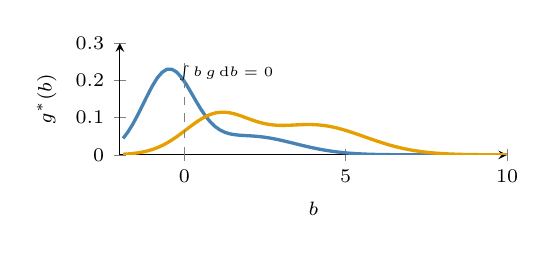
\begin{tikzpicture}
\begin{axis}[
    width=6.5cm, height=3cm,
    xlabel={$b$}, ylabel={$g^*(b)$},
    xmin=-2, xmax=10, ymin=0, ymax=0.3,
    axis lines=left, font=\scriptsize,
]
\addplot[softblue, very thick, domain=-1.9:10, samples=80]
    {0.22*exp(-(x+0.5)^2/1.2) + 0.05*exp(-(x-2)^2/4)};
\addplot[softorange, very thick, domain=-1.9:10, samples=80]
    {0.1*exp(-(x-1)^2/2) + 0.08*exp(-(x-4)^2/5)};
\draw[gray, dashed] (axis cs:0,0) -- (axis cs:0,0.25);
\node[font=\tiny] at (axis cs:1.3,0.22) {$\int b\,g\ud b = 0$};
\end{axis}
\end{tikzpicture}
\end{center}

\begin{itemize}\itemsep0pt\footnotesize
    \item Mean wealth $= 0$ (zero net supply)
    \item Large mass at $\ubar{b}$ (constrained)
    \item $q^* < \rho$ (low return)
\end{itemize}

\column{0.48\textwidth}
\begin{center}
\textbf{Aiyagari} (production economy)\\[2pt]
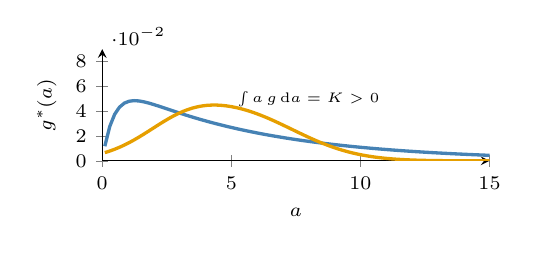
\begin{tikzpicture}
\begin{axis}[
    width=6.5cm, height=3cm,
    xlabel={$a$}, ylabel={$g^*(a)$},
    xmin=0, xmax=15, ymin=0, ymax=0.09,
    axis lines=left, font=\scriptsize,
]
\addplot[softblue, very thick, domain=0.1:15, samples=80]
    {0.065*exp(-0.18*(x-0.1)) * (1 - exp(-2*x))};
\addplot[softorange, very thick, domain=0.1:15, samples=80]
    {0.04*exp(-(x-5)^2/12) + 0.01*exp(-(x-3)^2/4)};
\node[font=\tiny] at (axis cs:8,0.05) {$\int a\,g\ud a = K > 0$};
\end{axis}
\end{tikzpicture}
\end{center}

\begin{itemize}\itemsep0pt\footnotesize
    \item Mean wealth $= K > 0$ (capital stock)
    \item Long right tail (wealthy agents)
    \item $r^* < \rho$ but capital earns return
\end{itemize}
\end{columns}

\vspace{0.1em}
{\footnotesize The PINN correctly captures these qualitative differences. Same code architecture, different market clearing conditions.}
\end{frame}

% --- Slide: Why PINNs over FD ---
\begin{frame}{Why PINNs over Finite Differences?}
\small
For stationary problems (Huggett/Aiyagari without aggregate shocks):

\vspace{0.1em}
\begin{center}
\footnotesize
\renewcommand{\arraystretch}{1.05}
\begin{tabular}{lcc}
\toprule
& \textbf{Finite Differences} & \textbf{PINN} \\
\midrule
Grid required & Yes ($I$ points) & \emphc{No} (collocation) \\
Upwind scheme & Manual implementation & Auto-diff handles it \\
Curse of dimensionality & $O(I^d)$ & $O(M \cdot |\theta|)$ \\
Extension to higher dim & Very hard & Natural \\
Borrowing constraint & Special treatment & Soft penalty / hard BC \\
Accuracy (2D) & $\sim 10^{-6}$ & $\sim 10^{-4}$ \\
Speed (2D) & Faster & Slower \\
\bottomrule
\end{tabular}
\end{center}

\vspace{0.1em}
\textbf{Verdict}: \textbf{\emph{FD is faster and more accurate}} for low-dim stationary problems --- use it as the gold-standard benchmark. PINNs \emphc{scale to high dimensions}: aggregate shocks (KS, state $\ni g$), multiple assets, richer heterogeneity.
\vspace{-0.2em}

$\Longrightarrow$ Part III: \textbf{EMINNs} for the master equation.
\end{frame}

% ============================================================================
% PART III: EMINNs FOR THE MASTER EQUATION
% ============================================================================

\section{EMINNs for the Master Equation}

\begin{frame}{}
\vfill
\begin{center}
{\Huge \textcolor{uzhblue}{\textbf{Part III}}}\\[12pt]
{\LARGE EMINNs: Solving the Master Equation}\\[6pt]
{\large Economic Model Informed Neural Networks}\\[6pt]
{\small Gu, Lauriere, Merkel \& Payne (2024)}\\[10pt]
{\footnotesize \textbf{Note:} the companion EMINN notebook is deferred to the next iteration of the course; this Part III is conceptual.}
\end{center}
\vfill
\end{frame}

% --- Slide: The Challenge ---
\begin{frame}{The Challenge: Aggregate Shocks}
\small
\textbf{Krusell--Smith} (1998): Add aggregate TFP shocks $dZ_t = \eta(\bar{Z}-Z_t)\ud t + \sigma^z\ud B_t^0$.

\vspace{0.2em}
Now the value function depends on the \emphc{entire distribution}:
\[
V = V(a, n, z, g) \qquad \text{where } g \text{ is infinite-dimensional}
\]

\vspace{0.1em}
\textbf{Why is this hard?}
\begin{itemize}\itemsep2pt
    \item Cannot discretize $g$ on a grid (infinite-dimensional)
    \item Original KS trick: $g \approx K$ (first moment). But loses distributional information.
    \item We want \emphc{global} solutions: accurate for all $(z, g)$, not just near steady state
\end{itemize}

\vspace{0.2em}
\begin{block}{The Master Equation (from Deck 1)}
\small
Substitute KFE + market clearing + belief consistency into HJB $\Rightarrow$ \emphc{single PDE}:
\[
\mathcal{L}V(a, n, z, g) = 0
\]
One PDE to solve, but with an infinite-dimensional argument $g$.
\end{block}
\end{frame}

% --- Slide: Three Approximations ---
\begin{frame}{Approximating the Distribution: Three Approaches}
\small
\textbf{Key idea}: Replace the infinite-dimensional $g$ by a \emphc{finite-dimensional} approximation $\hat{\varphi}$.

\vspace{0.2em}
\begin{center}
\small
\renewcommand{\arraystretch}{1.25}
\begin{tabular}{lccc}
\toprule
& \textbf{Finite Population} & \textbf{Discrete State} & \textbf{Projection} \\
\midrule
Dist.\ params $\hat{\varphi}_t$ & $\{(a_t^i, n_t^i)\}_{i\leq N}$ & Masses on grid & Basis coefficients \\[2pt]
Dist.\ approx.\ $\hat{g}_t$ & $\frac{1}{N}\sum \delta_{\hat{\varphi}_t^i}$ & $\sum \hat{\varphi}_{i,j,t}\delta_{(a_i,n_j)}$ & $b_0 + \sum \hat{\varphi}_{i,t}b_i(a,n)$ \\[2pt]
KFE approx. & Other agents' evolution & FD mass evolution & Coeff.\ evolution \\[2pt]
Dimension & $\sim 40$ & $\sim 200$ & $\sim 5$ \\[2pt]
$K_t =$ & $\frac{1}{N}\sum a_t^i$ & $\sum_j a_j \hat{\varphi}_{j,t}$ & $\int a \sum \hat{\varphi}_{i,t}b_i \ud a$ \\
\bottomrule
\end{tabular}
\end{center}

\vspace{0.2em}
\textbf{After approximation}: $V(a, n, z, g) \approx \hat{V}(a, n, z, \hat{\varphi})$ where $\hat{\varphi} \in \R^N$.

Now the master equation becomes a \emphc{finite-dimensional PDE} that a neural network can solve!
\end{frame}

% --- Slide: Finite Population ---
\begin{frame}{Approach 1: Finite Population ($N \approx 40$ agents)}
\small
Replace continuum by $N$ agents with states $\hat{\varphi}_t = \{(a_t^1, l_t^1), \ldots, (a_t^N, l_t^N)\}$.

\vspace{0.2em}
\textbf{Approximate capital}: $K_t = \frac{1}{N}\sum_{i=1}^N a_t^i$

\vspace{0.2em}
\textbf{Why are 40 agents sufficient?}
\begin{itemize}\itemsep2pt
    \item We sample individual states $(a,n)$ and distribution states $(\hat{\varphi})$ \emphc{separately} when generating training data
    \item For individual policy: can concentrate on high-curvature regions (near $\ubar{a}$) independently of $N$
    \item For aggregate capital: LLN kicks in quickly --- 40 agents give accurate $K$
    \item Can analytically eliminate finite-agent noise in $\hat{\varphi}$-drift during training
\end{itemize}

\vspace{0.2em}
\begin{center}
\colorbox{uzhgreylight}{\parbox{0.7\textwidth}{\centering\small
This is much smaller than discrete-time simulation methods\\
(e.g., Young's method from Day~4 used $\sim 10{,}000$ agents).\\
Continuous-time formulation helps!}}
\end{center}
\end{frame}

% --- Slide: Discrete State ---
\begin{frame}{Approach 2: Discrete State Space ($\sim 200$ grid points)}
\small
Discretize wealth on a grid $\{a_1, \ldots, a_I\}$. Distribution $\approx$ masses on grid:
\[
\hat{g}_t(a,n) \approx \sum_{i=1}^{I}\sum_{j=1}^{2} \hat{\varphi}_{i,j,t}\;\delta_{(a_i, n_j)}
\]

\vspace{0.1em}
\textbf{KFE becomes}: evolution of grid masses via \emphc{finite differences}.

\vspace{0.2em}
\textbf{Master equation}: functional derivative w.r.t.\ $g$ becomes a \emphc{partial derivative} w.r.t.\ each mass $\hat{\varphi}_{m,j}$:
\[
\hat{\mathcal{L}}_g \hat{W} = \sum_{j=1,2}\sum_{m=1}^{I} \mu_{\hat{\varphi},m,j}(z, \hat{\varphi})\;\partial_{\hat{\varphi}_{m,j}}\hat{W}
\]

\vspace{0.1em}
\textbf{Dimension}: $\hat{\varphi} \in \R^{2I}$ with $I \approx 100$, so $\dim(\hat{\varphi}) \approx 200$.

\vspace{0.2em}
\textbf{Neural network}: needs an \emphc{embedding} to handle the 200-dim input efficiently.\\
$\Rightarrow$ Use a recurrent or set-encoder architecture (Sirignano \& Spiliopoulos, 2018).
\end{frame}

% --- Slide: Projection ---
\begin{frame}{Approach 3: Projection onto Basis Functions ($\sim 5$ components)}
\small
\textbf{Idea}: Project $g$ onto a low-dimensional basis:
$\hat{g}_t(a,n) = b_0(a,n) + \sum_{i=1}^{N} \hat{\varphi}_{i,t}\,b_i(a,n)$

\vspace{0.2em}
\textbf{Choice of basis} (Gu et al., 2024):
\begin{itemize}\itemsep0pt
    \item Use \emphc{eigenfunctions} of the steady-state KFE operator $\bar{\mathcal{L}}^{KF}$
    \item These are the \emphc{most persistent} components of the density
    \item Intuition: most persistent components carry most price-relevant information
    \item Only $N \approx 5$ basis functions needed!
\end{itemize}

\vspace{0.1em}
\textbf{Dimension}: $\hat{\varphi} \in \R^5$. Total NN input: $(a, n, z, \hat{\varphi}) \in \R^{2+1+5} = \R^8$.

\vspace{0.1em}
\begin{center}
\colorbox{uzhgreylight}{\parbox{0.7\textwidth}{\centering\footnotesize
Projection is \emphc{lowest-dimensional} but requires the most intricate setup
(computing eigenfunctions, choosing test functions for KFE evolution).}}
\end{center}
\end{frame}

% --- Slide: Comparison of Approaches ---
\begin{frame}{Comparing the Three Approximation Approaches}
\small
\begin{center}
\small
\renewcommand{\arraystretch}{1.2}
\begin{tabular}{lccc}
\toprule
& \textbf{Finite Population} & \textbf{Discrete State} & \textbf{Projection} \\
\midrule
Dimension of $\hat{\varphi}$ & $\sim 40$ & $\sim 200$ & $\sim 5$ \\
NN architecture & Feed-forward & Recurrent + embedding & Feed-forward \\
Initialization & $W(a,\cdot) = e^{-a}$ & Random & Random \\
Customization & Choose $N$ & Grid, FD method & Basis, test functions \\
Conceptual difficulty & Low & Medium & High \\
\bottomrule
\end{tabular}
\end{center}

\vspace{0.3em}
\textbf{Trade-off}:
\begin{itemize}\itemsep1pt
    \item Finite population: simple concept, moderate dimension, works well in practice
    \item Discrete state: most similar to FD, highest dimension, needs embedding
    \item Projection: \emphc{lowest dimension}, but requires careful choice of basis and test functions
\end{itemize}

\vspace{0.2em}
{\small All three approaches are validated in Gu et al.\ (2024). They produce \emphc{consistent results}.}
\end{frame}

% --- Slide: Neural Network Parameterization ---
\begin{frame}{Neural Network for $W := \partial_a V$}
\small
\textbf{Parameterize} $W(\omega) \approx \hat{W}_\Theta(\omega)$ where $\omega = (a, n, z, \hat{\varphi})$:

\vspace{0.2em}
\begin{center}
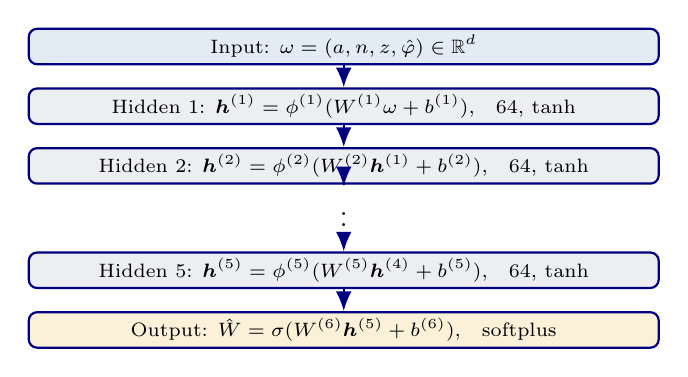
\begin{tikzpicture}[
    layer/.style={rectangle, rounded corners=3pt, draw=uzhblue, thick,
                  minimum width=8cm, minimum height=0.45cm, align=center,
                  font=\scriptsize, inner sep=2pt},
    arrow/.style={-{Latex[length=2.5mm,width=2mm]}, line width=0.8pt, uzhblue},
    node distance=0.28cm
]
\node[layer, fill=softblue!15]  (input)  {Input: $\omega = (a, n, z, \hat{\varphi}) \in \R^{d}$};
\node[layer, fill=uzhgreylight, below=of input]  (h1) {Hidden 1: $\bm{h}^{(1)} = \phi^{(1)}(W^{(1)}\omega + b^{(1)})$, \; 64, $\tanh$};
\node[layer, fill=uzhgreylight, below=of h1]     (h2) {Hidden 2: $\bm{h}^{(2)} = \phi^{(2)}(W^{(2)}\bm{h}^{(1)} + b^{(2)})$, \; 64, $\tanh$};
\node[font=\normalsize, below=0.02cm of h2]      (vd) {$\vdots$};
\node[layer, fill=uzhgreylight, below=0.05cm of vd] (h5) {Hidden 5: $\bm{h}^{(5)} = \phi^{(5)}(W^{(5)}\bm{h}^{(4)} + b^{(5)})$, \; 64, $\tanh$};
\node[layer, fill=softorange!15, below=of h5]    (output) {Output: $\hat{W} = \sigma(W^{(6)}\bm{h}^{(5)} + b^{(6)})$, \; softplus};

\draw[arrow] (input.south) -- (h1.north);
\draw[arrow] (h1.south)    -- (h2.north);
\draw[arrow] (h2.south)    -- (vd.north);
\draw[arrow] (vd.south)    -- (h5.north);
\draw[arrow] (h5.south)    -- (output.north);
\end{tikzpicture}
\end{center}

\vspace{0.1em}
\begin{itemize}\itemsep1pt
    \item $H = 5$ hidden layers, 64 neurons each, $\tanh$ activation
    \item Output: \emphc{softplus} $\sigma(x) = \log(1+e^x)$ ensures $W > 0$ (marginal value positive)
    \item Parameters: $\Theta = (W^{(1)}, b^{(1)}, \ldots, W^{(6)}, b^{(6)})$
    \item Optimal consumption: $c^* = W^{-1/\gamma}$ (directly from the envelope condition)
\end{itemize}
\end{frame}

% --- Slide: The EMINN Algorithm ---
\begin{frame}{The EMINN Algorithm}
\begin{block}{Economic Model Informed Neural Network (EMINN)}
\footnotesize
\begin{algorithmic}[1]
\STATE \textbf{Initialize} NN $\hat{W}_\Theta$ with parameters $\Theta$
\WHILE{Loss $>$ tolerance}
\STATE \textbf{Sample} $M$ points: $\bm{S} = (a_m, n_m, z_m, \hat{\varphi}_m)_{m=1}^M$
    \STATE \textbf{Compute} loss: $\mathcal{E} = \kappa^e\,\tfrac{1}{M}\sum_{m} |\hat{\mathcal{L}}(\cdot; \Theta)|^2 + \kappa^s\,\mathcal{E}^s(\bm{S}; \Theta)$
\STATE \quad $\hat{\mathcal{L}}$: master eq.\ residual (automatic differentiation); \; $\mathcal{E}^s$: shape penalty
    \STATE \textbf{Update} $\Theta \leftarrow \Theta - \alpha\,\nabla_\Theta\mathcal{E}$
\ENDWHILE
\end{algorithmic}
\end{block}

\vspace{0.2em}
\small
\textbf{This is exactly a PINN} applied to the master equation!
\begin{itemize}\itemsep0pt
    \item ``Physics'' $=$ economic equilibrium conditions (master equation)
    \item All derivatives (including w.r.t.\ $\hat{\varphi}$) computed by \emphc{automatic differentiation}
\end{itemize}
\end{frame}

% --- Slide: Master Equation Residual ---
\begin{frame}{Computing the Master Equation Residual}
\small
The residual $\hat{\mathcal{L}}$ decomposes into three operators:
\[
0 = (r(z,\hat{\varphi}) - \rho)\,\hat{W} + \underbrace{\hat{\mathcal{L}}_x\hat{W}}_{\text{individual}} + \underbrace{\hat{\mathcal{L}}_z\hat{W}}_{\text{TFP}} + \underbrace{\hat{\mathcal{L}}_g\hat{W}}_{\text{distribution}}
\]

\vspace{0.1em}
\begin{center}
\small
\renewcommand{\arraystretch}{1.3}
\begin{tabular}{ll}
\toprule
\textbf{Operator} & \textbf{Expression} \\
\midrule
$\hat{\mathcal{L}}_x\hat{W}$ & $s(\cdot)\partial_a\hat{W} + \lambda(n)\big(\hat{W}(\hat{n}) - \hat{W}(n)\big)$ \quad (savings + income switch) \\
$\hat{\mathcal{L}}_z\hat{W}$ & $\partial_z\hat{W}\cdot\mu^z(z) + \frac{1}{2}(\sigma^z)^2\partial_{zz}\hat{W}$ \quad (OU aggregate shock) \\
$\hat{\mathcal{L}}_g\hat{W}$ & $\sum_n \frac{\partial \hat{W}}{\partial \hat{\varphi}_n}\cdot\mu_{\hat{\varphi},n}(z, \hat{\varphi})$ \quad (distribution evolution) \\
\bottomrule
\end{tabular}
\end{center}

\vspace{0.2em}
\textbf{All derivatives} ($\partial_a, \partial_z, \partial_{zz}, \partial_{\hat{\varphi}_n}$) computed by \emphc{one backward pass} through the neural network.

\vspace{0.2em}
{\small This is the power of automatic differentiation: even the functional derivative (w.r.t.\ distribution) is just a partial derivative in the finite-dimensional approximation.}
\end{frame}

% --- Slide: Shape Constraints ---
\begin{frame}{Shape Constraints: Avoiding ``Cheat Solutions''}
\begin{alertblock}{The Macroeconomic Deep Learning Conundrum}
\footnotesize
The algorithm is straightforward to describe and code\ldots but \emphc{hard to implement successfully!}
NNs may get stuck in bad solutions (constant, non-increasing, non-concave $V$).
\end{alertblock}

\vspace{0.1em}
\small
\textbf{Solution}: Add \emphc{shape penalties} $\mathcal{E}^s$ to the loss:
\begin{itemize}\itemsep0pt
    \item \textbf{Concavity}: penalize $\partial_{aa}V > 0$: $\;\mathcal{E}^{\text{concav}} = \frac{1}{M}\sum \max(0, \partial_{aa}V_m)^2$
    \item \textbf{Monotonicity}: penalize $\partial_{za}V > 0$ (higher $z$ $\Rightarrow$ lower marginal value)
\end{itemize}

\vspace{0.1em}
\textbf{Additional tricks}:
\begin{itemize}\itemsep0pt
    \item \emphc{Initialization}: $W(a, \cdot) = e^{-a}$ (correct qualitative shape from the start)
    \item \emphc{Architecture}: train $\phi(a,n,z,g;\theta)\cdot(a-\ubar{a})^{1-\gamma}$ (correct asymptotics)
    \item \emphc{Active sampling}: sample more points where the residual is large
\end{itemize}
\end{frame}

% --- Slide: Sampling Strategies ---
\begin{frame}{Sampling Strategies: Where to Evaluate the Residual}
\small
\textbf{Challenge}: state space $(a, n, z, \hat{\varphi})$ is high-dimensional.
Must sample from \emphc{economically relevant} regions.

\vspace{0.1em}
\begin{columns}[T]
\column{0.50\textwidth}
\footnotesize
\textbf{Distribution $\hat{\varphi}$ sampling:}
\begin{enumerate}\itemsep0pt
    \item \emphc{Moment}: draw $K$, then $\hat{\varphi}$ consistent with $K$
    \item \emphc{Mixed steady-state}: solve SS for various $z$, take mixtures
    \item \emphc{Ergodic}: simulate economy with current $\hat{W}$, use simulated distributions
\end{enumerate}

\column{0.46\textwidth}
\footnotesize
\textbf{Individual states $(a, n)$:}
\begin{itemize}\itemsep0pt
    \item Uniform on $[\ubar{a}, \bar{a}] \times \{l_1, l_2\}$
    \item Add draws where error is high (\emphc{active sampling})
\end{itemize}

\vspace{0.1em}
\textbf{Aggregate state $z$:} Uniform on $[z_{\min}, z_{\max}]$
\end{columns}

\vspace{0.2em}
\begin{center}
\colorbox{uzhgreylight}{\parbox{0.85\textwidth}{\centering\small
\emphc{Separation of individual and distribution sampling} is key to efficiency.}}
\end{center}
\end{frame}

% --- Slide: Key Implementation Details ---
\begin{frame}{Implementation Details}
\scriptsize
\begin{center}
\renewcommand{\arraystretch}{1.0}
\begin{tabular}{lccc}
\toprule
& \textbf{Finite Pop.} & \textbf{Discrete State} & \textbf{Projection} \\
\midrule
\multicolumn{4}{l}{\textbf{Neural Network}} \\
\quad Structure & Feed-forward & RNN/embed. & Feed-forward \\
\quad Initialization & $W(a,\cdot) = e^{-a}$ & Random & Random \\
\multicolumn{4}{l}{\textbf{Sampling}} \\
\quad $(a, n)$ & Active & Uniform & Uniform \\
\quad $\hat{\varphi}$ & Moment sampling & Mixed steady-state & Ergodic \\
\quad $z$ & $U[z_{\min}, z_{\max}]$ & $U[z_{\min}, z_{\max}]$ & $U[z_{\min}, z_{\max}]$ \\
\multicolumn{4}{l}{\textbf{Loss Function}} \\
\quad Shape constraints & $\partial_{aa}V < 0$, $\partial_{za}V < 0$ & Same & $\partial_{aa}V < 0$ \\
\quad Weights & $\kappa^e = 100$, $\kappa^s = 1$ & $\kappa^e = \kappa^s = 1$ & $\kappa^e = \kappa^s = 1$ \\
\bottomrule
\end{tabular}
\end{center}

\vspace{0.05em}
\footnotesize
\textbf{Q\&A: Key differences from discrete time (Day 2--4)?}
\begin{itemize}\itemsep0pt
    \item Derivatives replace expectations, so automatic differentiation is essential.
    \item Collocation and shape constraints replace simulation grids and false-time steps.
\end{itemize}
\end{frame}

% ============================================================================
% PART IV: RESULTS AND OUTLOOK
% ============================================================================

\section{Results, Comparison, and Outlook}

\begin{frame}{}
\vfill
\begin{center}
{\Huge \textcolor{uzhblue}{\textbf{Part IV}}}\\[12pt]
{\LARGE Results, Comparison, and Outlook}
\end{center}
\vfill
\end{frame}

% --- Slide: Aiyagari Results ---
\begin{frame}[shrink=2]{Results: Aiyagari Model (No Aggregate Shocks)}
\small
\textbf{Validation}: Compare EMINN solutions against finite-difference benchmark.

\vspace{0.1em}
\begin{columns}[T]
\column{0.50\textwidth}
\begin{center}
\footnotesize
\renewcommand{\arraystretch}{1.1}
\begin{tabular}{lcc}
\toprule
\textbf{Method} & \textbf{ME Loss} & \textbf{MSE(NN,FD)} \\
\midrule
Finite Pop.\ NN & $3.1 \times 10^{-5}$ & $4.8 \times 10^{-5}$ \\
Discrete State NN & $9.3 \times 10^{-6}$ & $6.6 \times 10^{-5}$ \\
\bottomrule
\end{tabular}
\end{center}

\vspace{0.1em}
\begin{itemize}\itemsep0pt
    \item ME residual: $\sim 10^{-5}$ (excellent)
    \item Agreement with FD: $\sim 10^{-5}$ MSE
    \item Both approaches match FD closely
    \item Consistent across multiple runs
\end{itemize}

\column{0.47\textwidth}
\begin{center}
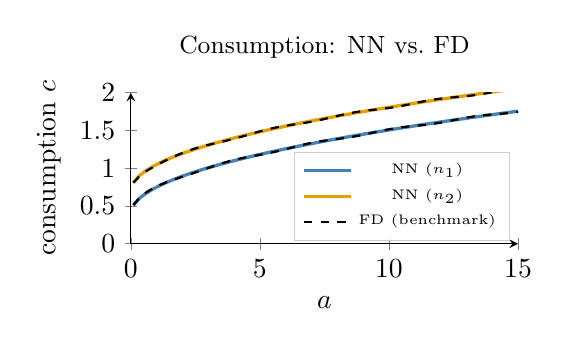
\begin{tikzpicture}
\begin{axis}[
    width=6.5cm, height=3.5cm,
    xlabel={$a$}, ylabel={consumption $c$},
    xmin=0, xmax=15, ymin=0, ymax=2,
    axis lines=left,
    legend style={at={(0.98,0.02)}, anchor=south east, font=\tiny,
                  fill=white, fill opacity=0.85, draw=gray!40, text opacity=1},
    title={\small Consumption: NN vs.\ FD},
    title style={at={(0.5,1.05)}, font=\small},
]
% NN solution
\addplot[softblue, very thick, domain=0.1:15, samples=60]
    {0.4 + 0.35*sqrt(x)};
\addlegendentry{NN ($n_1$)}
\addplot[softorange, very thick, domain=0.1:15, samples=60]
    {0.7 + 0.35*sqrt(x)};
\addlegendentry{NN ($n_2$)}
% FD solution
\addplot[black, thick, dashed, domain=0.1:15, samples=60]
    {0.4 + 0.35*sqrt(x) + 0.01*sin(deg(2*x))};
\addlegendentry{FD (benchmark)}
\addplot[black, thick, dashed, domain=0.1:15, samples=60]
    {0.7 + 0.35*sqrt(x) - 0.01*sin(deg(2*x))};
\end{axis}
\end{tikzpicture}
\end{center}
\end{columns}
\end{frame}

% --- Slide: Aiyagari Plots ---
\begin{frame}[shrink=2]{Aiyagari: Consumption, Marginal Value, and Distribution}
\begin{columns}[T]
\column{0.32\textwidth}
\begin{center}
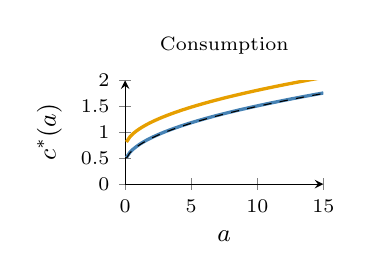
\begin{tikzpicture}
\begin{axis}[
    width=4.1cm, height=2.9cm,
    xlabel={\small $a$}, ylabel={\small $c^*(a)$},
    xmin=0, xmax=15, ymin=0, ymax=2,
    axis lines=left, font=\scriptsize,
    title={\scriptsize Consumption},
    legend style={at={(0.02,0.98)}, anchor=north west, font=\tiny},
]
\addplot[softblue, very thick, domain=0.1:15, samples=60]
    {0.4 + 0.35*sqrt(x)};
\addplot[softorange, very thick, domain=0.1:15, samples=60]
    {0.7 + 0.35*sqrt(x)};
\addplot[black, dashed, thin, domain=0.1:15, samples=60]
    {0.39 + 0.35*sqrt(x)};
\end{axis}
\end{tikzpicture}
\end{center}

\column{0.32\textwidth}
\begin{center}
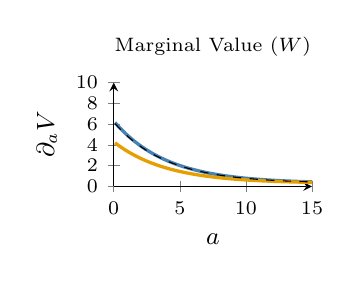
\begin{tikzpicture}
\begin{axis}[
    width=4.1cm, height=2.9cm,
    xlabel={\small $a$}, ylabel={\small $\partial_a V$},
    xmin=0, xmax=15, ymin=0, ymax=10,
    axis lines=left, font=\scriptsize,
    title={\scriptsize Marginal Value ($W$)},
]
\addplot[softblue, very thick, domain=0.1:15, samples=60]
    {6*exp(-0.25*x) + 0.3};
\addplot[softorange, very thick, domain=0.1:15, samples=60]
    {4*exp(-0.25*x) + 0.3};
\addplot[black, dashed, thin, domain=0.1:15, samples=60]
    {5.9*exp(-0.25*x) + 0.3};
\end{axis}
\end{tikzpicture}
\end{center}

\column{0.32\textwidth}
\begin{center}
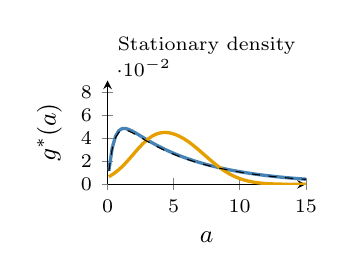
\begin{tikzpicture}
\begin{axis}[
    width=4.1cm, height=2.9cm,
    xlabel={\small $a$}, ylabel={\small $g^*(a)$},
    xmin=0, xmax=15, ymin=0, ymax=0.09,
    axis lines=left, font=\scriptsize,
    title={\scriptsize Stationary density},
]
\addplot[softblue, very thick, domain=0.1:15, samples=60]
    {0.065*exp(-0.18*(x-0.1)) * (1 - exp(-2*x))};
\addplot[softorange, very thick, domain=0.1:15, samples=60]
    {0.04*exp(-(x-5)^2/12) + 0.01*exp(-(x-3)^2/4)};
\addplot[black, dashed, thin, domain=0.1:15, samples=60]
    {0.063*exp(-0.18*(x-0.1)) * (1 - exp(-2*x))};
\end{axis}
\end{tikzpicture}
\end{center}
\end{columns}

\vspace{0.1em}
\begin{center}
{\scriptsize Solid curves: NN \qquad Dashed curves: FD benchmark}
\end{center}

\vspace{0.1em}
{\small NN and FD are very close across all three panels.}
\end{frame}

% --- Slide: Krusell-Smith Results ---
\begin{frame}{Reported Results: Krusell--Smith with Aggregate Shocks}
\footnotesize
\textbf{Gu et al.\ (2024)} report global master-equation solutions with aggregate TFP shocks.

\vspace{0.1em}
\begin{center}
\footnotesize
\renewcommand{\arraystretch}{1.1}
\begin{tabular}{lc}
\toprule
\textbf{Method} & \textbf{Master Eq.\ Training Loss} \\
\midrule
Finite Pop.\ NN & $3.0 \times 10^{-5}$ \\
Discrete Grid NN & $9.6 \times 10^{-5}$ \\
Projection NN & $8.5 \times 10^{-6}$ \\
\bottomrule
\end{tabular}
\end{center}

\vspace{0.15em}
All three approaches achieve reported training losses around $10^{-5}$.

\vspace{0.1em}
\textbf{Comparison with Fernandez-Villaverde, Hurtado \& Nuno (2023):}
\begin{itemize}\itemsep1pt
    \item Their method: perturbation around steady state
    \item EMINN: neural global approximation of the master equation
    \item Reported paths match closely for moderate shocks; differences matter farther from steady state
\end{itemize}
\end{frame}

% --- Slide: KS Time Paths ---
\begin{frame}{Krusell--Smith: Sample Time Paths}
\begin{columns}[T]
\column{0.48\textwidth}
\begin{center}
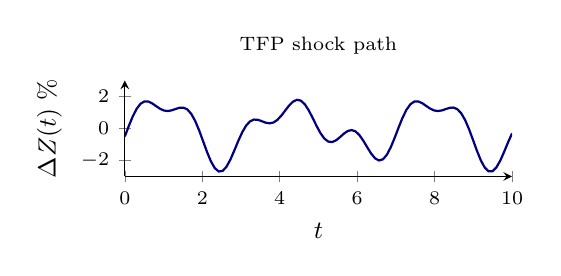
\begin{tikzpicture}
\begin{axis}[
    width=6.5cm, height=2.8cm,
    xlabel={\small $t$}, ylabel={\small $\Delta Z(t)$ \%},
    xmin=0, xmax=10, ymin=-3, ymax=3,
    axis lines=left, font=\scriptsize,
    title={\scriptsize TFP shock path},
]
\addplot[uzhblue, thick, domain=0:10, samples=100]
    {1.5*sin(deg(1.8*x)) + 0.8*sin(deg(4.5*x)) - 0.5*cos(deg(2.7*x))};
\end{axis}
\end{tikzpicture}

\vspace{-0.1em}
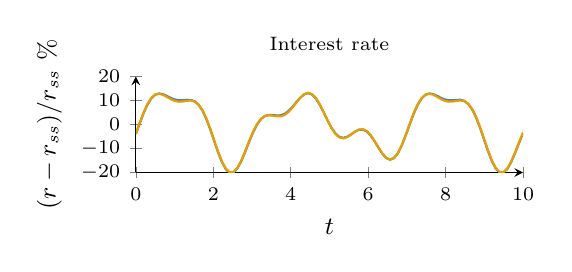
\begin{tikzpicture}
\begin{axis}[
    width=6.5cm, height=2.8cm,
    xlabel={\small $t$}, ylabel={\small $(r - r_{ss})/r_{ss}$ \%},
    xmin=0, xmax=10, ymin=-20, ymax=20,
    axis lines=left, font=\scriptsize,
    title={\scriptsize Interest rate},
]
\addplot[softblue, thick, domain=0:10, samples=100]
    {12*sin(deg(1.8*x)) + 5*sin(deg(4.5*x)) - 4*cos(deg(2.7*x))};
\addplot[softorange, thick, domain=0:10, samples=100]
    {11.8*sin(deg(1.8*x)) + 5.2*sin(deg(4.5*x)) - 3.8*cos(deg(2.7*x))};
\end{axis}
\end{tikzpicture}
\end{center}

\column{0.48\textwidth}
\begin{center}
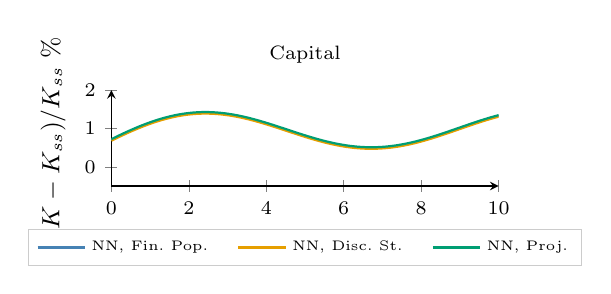
\begin{tikzpicture}
\begin{axis}[
    width=6.5cm, height=2.8cm,
    xlabel={\small $t$}, ylabel={\small $(K - K_{ss})/K_{ss}$ \%},
    xmin=0, xmax=10, ymin=-0.5, ymax=2,
    axis lines=left, font=\scriptsize,
    title={\scriptsize Capital},
    legend columns=3,
    legend style={at={(0.5,-0.45)}, anchor=north, font=\tiny,
                  draw=gray!40, /tikz/every even column/.append style={column sep=0.3cm}},
]
\addplot[softblue, thick, domain=0:10, samples=100]
    {0.7 + 0.5*sin(deg(0.7*x)) + 0.3*(1-exp(-0.5*x))};
\addlegendentry{NN, Fin.~Pop.}
\addplot[softorange, thick, domain=0:10, samples=100]
    {0.68 + 0.5*sin(deg(0.7*x)) + 0.3*(1-exp(-0.5*x))};
\addlegendentry{NN, Disc.~St.}
\addplot[softgreen, thick, domain=0:10, samples=100]
    {0.72 + 0.5*sin(deg(0.7*x)) + 0.3*(1-exp(-0.5*x))};
\addlegendentry{NN, Proj.}
\end{axis}
\end{tikzpicture}

\vspace{-0.1em}
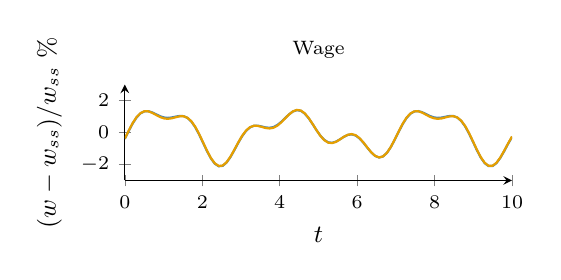
\begin{tikzpicture}
\begin{axis}[
    width=6.5cm, height=2.8cm,
    xlabel={\small $t$}, ylabel={\small $(w - w_{ss})/w_{ss}$ \%},
    xmin=0, xmax=10, ymin=-3, ymax=3,
    axis lines=left, font=\scriptsize,
    title={\scriptsize Wage},
]
\addplot[softblue, thick, domain=0:10, samples=100]
    {1.2*sin(deg(1.8*x)) + 0.6*sin(deg(4.5*x)) - 0.4*cos(deg(2.7*x))};
\addplot[softorange, thick, domain=0:10, samples=100]
    {1.18*sin(deg(1.8*x)) + 0.62*sin(deg(4.5*x)) - 0.38*cos(deg(2.7*x))};
\end{axis}
\end{tikzpicture}
\end{center}
\end{columns}

\vspace{0.1em}
{\small All three NN approaches produce \emphc{nearly identical} time paths for aggregate variables.}
\end{frame}

% --- Slide: Method Comparison ---
\begin{frame}{Method Comparison: FD vs.\ PINN vs.\ EMINN}
\footnotesize
\begin{center}
\scriptsize
\renewcommand{\arraystretch}{1.12}
\begin{tabular}{lccc}
\toprule
& \textbf{Finite Diff.} & \textbf{PINN} & \textbf{EMINN} \\
\midrule
Global master eq. & \textcolor{darkred}{\ding{55}} & \textcolor{darkred}{\ding{55}} & \textcolor{darkgreen}{\ding{51}} \\
Stationary equilibrium & \textcolor{darkgreen}{\ding{51}} & \textcolor{darkgreen}{\ding{51}} & \textcolor{darkgreen}{\ding{51}} \\
Grid required & Yes & No & No \\
High-dimensional scaling & Limited & Better, validate & Better, validate \\
Handles $g$ as state & Standard: no & No & Via $\hat{\varphi}$ \\
Theory & Strong in low dim & Limited & Limited \\
Low-dim accuracy & $\sim 10^{-6}$ & problem-dependent & reported $\sim 10^{-5}$ \\
\bottomrule
\end{tabular}
\end{center}

\vspace{0.1em}
\textbf{Bottom line:}
\begin{itemize}\itemsep0pt
    \item \textbf{Stationary, low-dim}: FD is fast and reliable. Use it as benchmark.
    \item \textbf{Aggregate shocks}: EMINNs target global master-equation solutions.
    \item \textbf{PINNs}: useful bridge for the coupled HJB--KFE system.
\end{itemize}
\end{frame}

% --- Slide: The Deep Learning Advantage ---
\begin{frame}{The Deep Learning Advantage}
\small
\begin{columns}[T]
\column{0.48\textwidth}
\textbf{Why deep learning for het.\ agent macro?}
\begin{enumerate}\itemsep2pt
    \item \emphc{Meshless}: no exponential grid growth
    \item \emphc{Handles $\infty$-dim states}: distribution $g$ approximated by finite $\hat{\varphi}$, NN handles the rest
    \item \emphc{Auto-diff}: all derivatives (incl.\ functional) computed automatically
    \item \emphc{Global}: accurate for all states, not just near steady state
    \item \emphc{Flexible}: same framework for Huggett, Aiyagari, KS, HANK, \ldots
\end{enumerate}

\column{0.48\textwidth}
\textbf{Connection to this course:}
\begin{center}
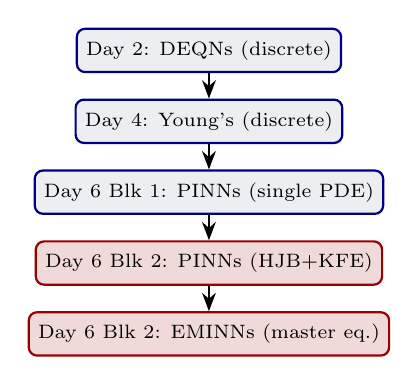
\begin{tikzpicture}[
    box/.style={rectangle, rounded corners=3pt, draw=uzhblue, thick, fill=uzhgreylight, minimum width=3.3cm, minimum height=0.55cm, align=center, font=\scriptsize},
    current/.style={box, fill=harvardcrimson!15, draw=harvardcrimson},
    arrow/.style={-Stealth, thick}
]
\node[box] (d2) at (0,3.5) {Day 2: DEQNs (discrete)};
\node[box] (d4) at (0,2.6) {Day 4: Young's (discrete)};
\node[box] (d5) at (0,1.7) {Day 6 Blk 1: PINNs (single PDE)};
\node[current] (d6a) at (0,0.8) {Day 6 Blk 2: PINNs (HJB+KFE)};
\node[current] (d6b) at (0,-0.1) {Day 6 Blk 2: EMINNs (master eq.)};

\draw[arrow] (d2) -- (d4);
\draw[arrow] (d4) -- (d5);
\draw[arrow] (d5) -- (d6a);
\draw[arrow] (d6a) -- (d6b);
\end{tikzpicture}
\end{center}
\end{columns}
\end{frame}

% --- Slide: Open Challenges ---
\begin{frame}{Open Challenges}
\begin{alertblock}{The Macroeconomic Deep Learning Conundrum (Gu et al., 2024)}
\small
``The algorithm is straightforward to describe and code\ldots but hard to implement successfully!''
\end{alertblock}

\vspace{0.2em}
\small
\textbf{Key challenges:}
\begin{enumerate}\itemsep2pt
    \item \textbf{Training stability}: NN can get stuck in bad local minima (``cheat solutions'')
    \begin{itemize}\itemsep0pt
        \item Constant, non-increasing, or non-concave $V$ $\Rightarrow$ shape penalties needed
    \end{itemize}
    \item \textbf{No convergence guarantees}: unlike FD, we cannot prove the NN converges
    \item \textbf{Sensitivity to hyperparameters}: architecture, lr, sampling, loss weights all matter
    \item \textbf{Verification}: \emphc{must} compare against known solutions (FD, perturbation)
    \begin{itemize}\itemsep0pt
        \item First validate on Aiyagari (no agg.\ shocks), then extend to KS
    \end{itemize}
    \item \textbf{Computational cost}: training can take hours/days on GPU for large models
\end{enumerate}

\vspace{0.2em}
{\small Active research area: better architectures, better sampling, better loss functions.}
\end{frame}

% --- Slide: Extensions ---
\begin{frame}{Extensions and Future Directions}
\small
The EMINN framework extends naturally to richer models:

\vspace{0.2em}
\begin{columns}[T]
\column{0.48\textwidth}
\textbf{Model extensions:}
\begin{itemize}\itemsep1pt
    \item \textbf{HANK}: add nominal rigidities\\
    {\small (Kaplan, Moll \& Violante, 2018)}
    \item \textbf{Multi-asset}: bonds + stocks + housing\\
    {\small (higher-dim individual state)}
    \item \textbf{Life-cycle}: age as additional state\\
    {\small (more heterogeneity)}
    \item \textbf{Non-convex adjustment costs}\\
    {\small (e.g., lumpy investment)}
\end{itemize}

\column{0.48\textwidth}
\textbf{Methodological extensions:}
\begin{itemize}\itemsep1pt
    \item \textbf{Better sampling}: importance sampling, adaptive collocation
    \item \textbf{Transfer learning}: pre-train on simpler model, fine-tune on complex one
    \item \textbf{Multi-scale training}: curriculum from easy $\to$ hard
    \item \textbf{Hybrid FD-NN}: use FD for low-dim parts, NN for high-dim parts
\end{itemize}
\end{columns}

\vspace{0.3em}
\begin{center}
\colorbox{uzhgreylight}{\parbox{0.8\textwidth}{\centering\small
\textbf{The frontier}: Can we solve HANK models with aggregate shocks \emphc{globally}?\\
This is one of the most important open problems in computational macro.}}
\end{center}
\end{frame}

% --- Slide: Summary ---
\begin{frame}{Summary and Key Takeaways}
\begin{columns}[T]
\column{0.32\textwidth}
\begin{block}{FD (Benchmark)}
\centering\small
\vspace{0.1em}
Fast and accurate for \emphc{stationary, low-dim} problems. Gold standard for Aiyagari/Huggett.
\vspace{0.1em}
\end{block}

\column{0.32\textwidth}
\begin{block}{PINN (Coupled PDEs)}
\centering\small
\vspace{0.1em}
\emphc{Mesh-free} solution of HJB + KFE via auto-diff. Same philosophy as Day~5.
\vspace{0.1em}
\end{block}

\column{0.32\textwidth}
\begin{block}{EMINN (Master Eq.)}
\centering\small
\vspace{0.1em}
\emphc{Global solutions} with aggregate shocks. Handles distribution as state.
\vspace{0.1em}
\end{block}
\end{columns}

\vspace{0.2em}
\small
\textbf{The big picture:}
\begin{enumerate}\itemsep0pt
    \item CT het.\ agent models $=$ coupled HJB + KFE + market clearing
    \item Deep learning (PINNs/EMINNs) embeds equilibrium conditions in the loss
    \item Auto-differentiation computes all derivatives (including functional derivatives)
    \item For aggregate shocks: approximate $g$ in finite dimensions, solve master equation
    \item Validated against FD benchmarks --- works, but training requires care
\end{enumerate}

\vspace{0.1em}
\begin{center}
\textbf{Tomorrow}: Surrogate models \& Gaussian Processes (Day~7).
\end{center}
\end{frame}

% --- Slide: Code Companion ---
\begin{frame}{Code Companion: Run This Live}
\footnotesize
\textbf{Day 6 companion notebooks (self-contained, PyTorch):}
\begin{itemize}\itemsep2pt
    \item \textbf{NB 06} \textit{(self-study)}: \texttt{06\_PE\_Discrete\_HJB\_PINN.ipynb} --- 1D PE with discrete income: upwind FD + PINN
    \item \textbf{NB 07} \textit{(self-study)}: \texttt{07\_PE\_Diffusion\_HJB\_PINN.ipynb} --- 2D PE with OU earnings: 2D FD + PINN
    \item \textbf{NB 08} \textit{(in-class)}: \texttt{08\_Aiyagari\_Continuous\_Time\_FD\_and\_PINN\_PyTorch.ipynb} --- full GE Aiyagari: HJB + KFE + market clearing
\end{itemize}

\vspace{0.2em}
\textbf{Suggested in-class demo flow:}
\begin{enumerate}\itemsep1pt
    \item Start with NB~06 (simplest, self-study): FD convergence, then PINN overlay
    \item Move to NB~07 (self-study): 2D contour plots, cross-sections, mesh-free advantage
    \item Focus on NB~08 (in-class): full GE loop, PINN vs FD agreement diagnostics
\end{enumerate}
\end{frame}

% --- Slide: References ---
\begin{frame}{References}
\tiny
\begin{columns}[T]
\column{0.48\textwidth}
\textbf{Core papers:}
\begin{itemize}\itemsep0pt
    \item Achdou, Y., Han, J., Lasry, J.-M., Lions, P.-L.\ \& Moll, B.\ (2022). Income and Wealth Distribution in Macroeconomics: A CT Approach. \emph{REStud} 89(1), 45--86.
    \item Gu, Z., Lauriere, M., Merkel, S.\ \& Payne, J.\ (2024). Global Solutions to Master Equations for CT HA Models. arXiv:2406.13726.
    \item Fernandez-Villaverde, J., Hurtado, S.\ \& Nuno, G.\ (2023). Financial Frictions and the Wealth Distribution. \emph{Econometrica} 91(3), 869--901.
\end{itemize}

\vspace{0.1em}
\textbf{Foundational:}
\begin{itemize}\itemsep0pt
    \item Aiyagari, S.R.\ (1994). Uninsured Idiosyncratic Risk and Aggregate Saving. \emph{QJE} 109(3), 659--684.
    \item Huggett, M.\ (1993). The Risk-Free Rate in HA Economies. \emph{JEDC} 17(5--6), 953--969.
    \item Krusell, P.\ \& Smith, A.A.\ (1998). Income and Wealth Heterogeneity. \emph{JPE} 106(5), 867--896.
\end{itemize}

\column{0.48\textwidth}
\textbf{Mean field games and DL:}
\begin{itemize}\itemsep0pt
    \item Lasry, J.-M.\ \& Lions, P.-L.\ (2007). Mean Field Games. \emph{Jpn.\ J.\ Math.}\ 2(1), 229--260.
    \item Sirignano, J.\ \& Spiliopoulos, K.\ (2018). DGM: A Deep Learning Algorithm for Solving PDEs. \emph{J.\ Comput.\ Phys.}\ 375, 1339--1364.
\end{itemize}

\vspace{0.1em}
\textbf{HANK and applications:}
\begin{itemize}\itemsep0pt
    \item Kaplan, G., Moll, B.\ \& Violante, G.L.\ (2018). Monetary Policy According to HANK. \emph{AER} 108(3), 697--743.
    \item Ahn, S., Kaplan, G., Moll, B., Winberry, T.\ \& Wolf, C.\ (2018). When Inequality Matters for Macro. \emph{NBER Macro Annual} 32(1), 1--75.
    \item Gabaix, X., Lasry, J.-M., Lions, P.-L.\ \& Moll, B.\ (2016). The Dynamics of Inequality. \emph{Ecta} 84(6), 2071--2111.
    \item Nuno, G.\ \& Moll, B.\ (2018). Social Optima in Economies with HA. \emph{RED} 28, 150--180.
\end{itemize}

\vspace{0.1em}
\textbf{Moll lecture notes:}
\begin{itemize}\itemsep0pt
    \item \url{benjaminmoll.com/lectures/} and \url{benjaminmoll.com/codes/}
\end{itemize}
\end{columns}
\end{frame}

% --- Slide: Questions ---
\begin{frame}{}
\begin{columns}[c]
\column{0.45\textwidth}
\begin{center}
{\Huge \textcolor{uzhblue}{\textbf{Questions?}}}

\vspace{1.0cm}
{\large Simon Scheidegger}\\[4pt]
{\small HEC, University of Lausanne}\\[4pt]
\url{https://sischei.github.io}

\vspace{0.6cm}
{\small Materials:~~\url{https://github.com/sischei/Deep_Learning_for_Solving_And_Estimating_Dynamic_Economic_Models}}
\end{center}

\column{0.45\textwidth}
\begin{center}
\textbf{Covered today (Deck 2):}\\[8pt]
{\small
\begin{tabular}{rl}
I & FD: The Benchmark \\
II & PINNs for HJB+KFE \\
III & EMINNs for Master Eq. \\
IV & Results \& Outlook \\
\end{tabular}
}

\vspace{0.8cm}
\textbf{Tomorrow (Day 7):}\\[6pt]
{\large Surrogate Models}\\
{\large \& Gaussian Processes}\\[8pt]
{\small 09:00--12:00}
\end{center}
\end{columns}
\end{frame}

\end{document}
